% Estas slides tienen que abrirse con el programa pdfpc que soporta videos embebidos
% el comando es: pdfpc -g slides.pdf
% para los videos se requiere ubuntu-restricted-extras


%\documentclass[compress,handout]{beamer}
\documentclass[compress]{beamer}
% compress pone la seccion abajo de todo
\mode<presentation>


% Theme customization
\usetheme{Copenhagen}
\useoutertheme{taihu}
%\useinnertheme{rectangles}
\setbeamertemplate{itemize item}[rectangle] % configure itemize
\setbeamertemplate{itemize subitem}[circle] % configure itemize
\setbeamertemplate{itemize subsubitem}[triangle] % configure itemize
\setbeamertemplate{navigation symbols}{} % remover simbolos e navegacion de las slides
\usefonttheme[onlymath]{serif} % simbolos matematicos en serif (Como es en latex original)

\setbeamertemplate{blocks}[rounded] % blocks corners rounded
\setbeamercolor{block body}{bg=blue!12,fg=black} % color of blocks

% Latex packages
\usepackage{pdfpc-commands} % pdfpc movie commands
\usepackage[utf8]{inputenc}
\usepackage[spanish]{babel}
\usepackage[binary-units=true]{siunitx} % para manejar las unidades
\usepackage{multirow}
\usepackage{multimedia}
\usepackage{graphicx}
\usepackage{xcolor}
\usepackage{booktabs} % \toprule
\usepackage[caption=false]{subfig} % caption = false elimina la palabra "Figura" del caption
\setbeamertemplate{caption}{\raggedright\insertcaption\par} % elimina la palabra "Figura" del caption
\usepackage{import} % para el comando import (se usa para pdf_tex)
\captionsetup[subfigure]{labelformat=empty} % remover el indice del caption de la subfigura

% add math preamble
\usepackage{amsmath}
\usepackage{amssymb}
\usepackage{amsopn}

% math
\renewcommand{\vec}[1]{\boldsymbol{\mathbf{#1}}}
\newcommand{\norm}[1]{\left\lVert#1\right\rVert}

% Declare arg max and arg min functionss
\DeclareMathOperator*{\argmax}{arg\,max}
\DeclareMathOperator*{\argmin}{arg\,min}

% Homogeneous decoration function
\newcommand{\homo}[1]{\dot{#1}}

% Declare projection as math function
\DeclareMathOperator{\proj}{proj}
\DeclareMathOperator{\disp}{disp}
\newcommand{\worldCoordSystem}{\mathrm{w}}
\newcommand{\cameraCoordSystem}{\mathrm{c}}
\newcommand{\point}{\vec{x}}
\newcommand{\worldPoint}{\point^{\mathrm{w}}}
\newcommand{\homoWorldPoint}{\homo{\point}^{\mathrm{w}}}
\newcommand{\cameraPoint}{\point^{\mathrm{c}}}
\newcommand{\hatCameraPoint}{\hat{\point}^{\mathrm{c}}}
\newcommand{\homoCameraPoint}{\homo{\point}^{\mathrm{c}}}
\newcommand{\measurement}{\vec{z}}
\newcommand{\prediction}{\hat{\vec{z}}}
\newcommand{\imagePoint}{\vec{u}}
\newcommand{\seMatrix}{\vec{E}}
\newcommand{\rotation}{\vec{R}}
\newcommand{\translation}{\vec{t}}
\newcommand{\intrinsicMatrix}{\vec{K}}
\newcommand{\principalPoint}{\vec{c}}
\newcommand{\reprojectionError}{u}
\newcommand{\projectionMatrix}{\vec{P}}
\newcommand{\cameraCenter}{\vec{o}}


% Dense Map
\newcommand{\current}{\mathrm{current}}
\newcommand{\previous}{\mathrm{previous}}
\newcommand{\fusion}{\mathrm{fusion}}
\newcommand{\inverseDepth}{\rho}
\newcommand{\plane}{\boldsymbol{\pi}}
\newcommand{\reference}{ref}


% scaled operators and letters to fancy view
\newcommand{\sminus}{\scalebox{0.5}[1.0]{$-$}}
\newcommand{\splus}{\scalebox{0.6}[0.6]{$+$}}
\newcommand{\curr}{c}
\newcommand{\sind}[1]{\scalebox{0.6}[0.6]{$#1$}}
\newcommand{\ind}[1]{\scalebox{0.7}[0.7]{$#1$}}

\newcommand{\keyframe}{\vec{K}}
\newcommand{\pointCloud}{\mathcal P}
\newcommand{\groundTruth}[1]{{#1}^{*}}

\newcommand{\update}[1]{\hat{#1}}

\newcommand{\position}{\vec{p}}
\newcommand{\map}{M}

\newcommand{\baseline}{b}
\newcommand{\focalDistance}{f}
\newcommand{\disparityMap}{\mathcal D}
\newcommand{\camera}{c}
\newcommand{\ray}{n}




\setbeamerfont{title}{size=\large}
\title{Hacia una densificación de sistemas SLAM	dispersos basados en visión estéreo}
\author{Ariel D'Alessandro \and \underline{Taihú Pire} \and Rodrigo Baravalle}
\institute{	CIFASIS - CONICET - UNR}
\date{\scriptsize{Noviembre 17, 2017}}


\begin{document}

\frame{\titlepage}

\section{S-PTAM}

\begin{frame}
	\frametitle{S-PTAM en acción!}
	\centering
	
	\inlineMovie[loop&autostart&start=10]{./videos/kitti_lc.mkv}{./images/portada-sptam-kitti-video}{width=\columnwidth}
\end{frame}


\section{Dense S-PTAM}

\begin{frame}
	\frametitle{Dense S-PTAM}
	\begin{figure}[htb]
		\centering
		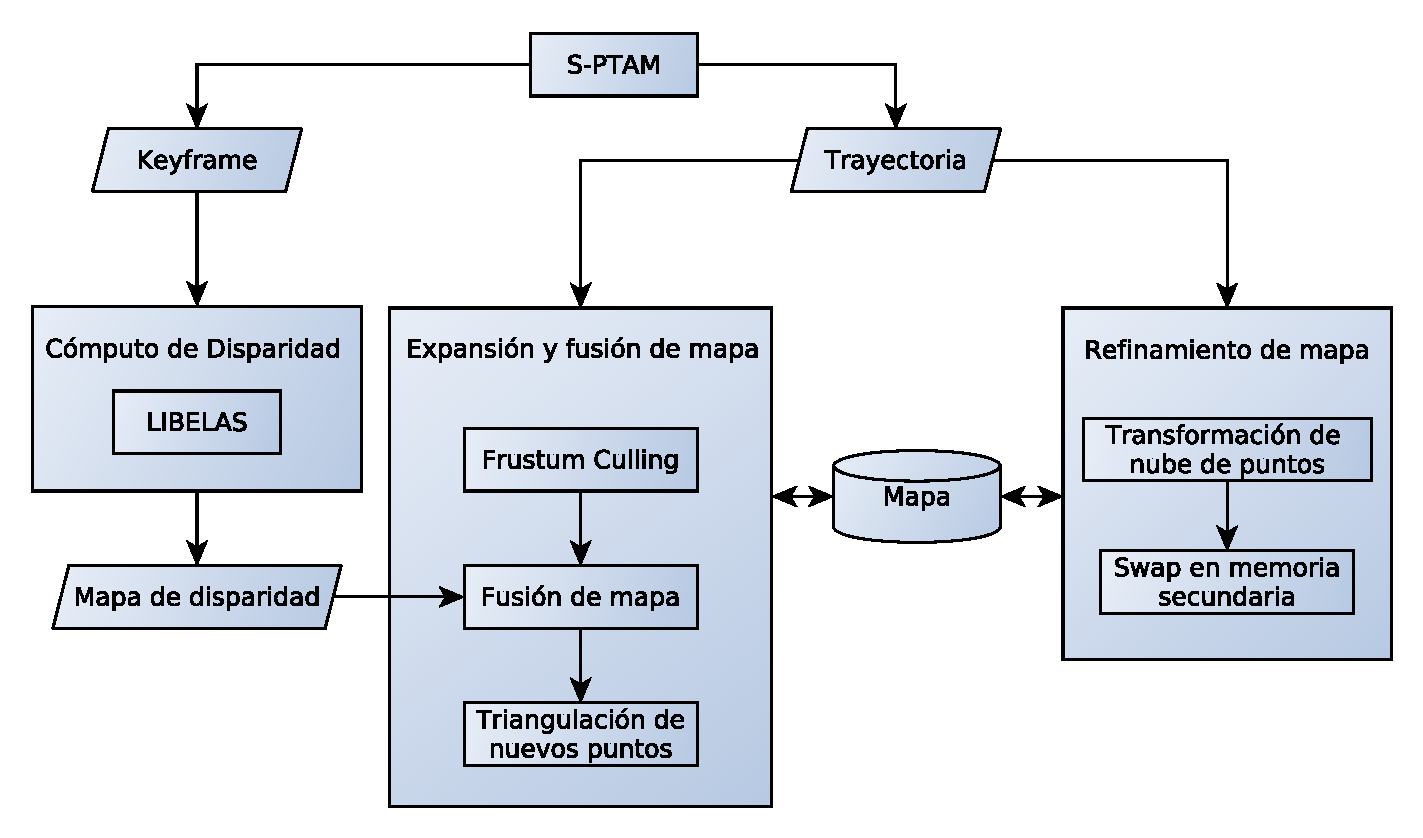
\includegraphics[width=\columnwidth]{images/dense_diagram.pdf}
	\end{figure}
\end{frame}

\begin{frame}
	\frametitle{Heurística de fusión de puntos}
	\begin{figure}[htb]
		\centering
		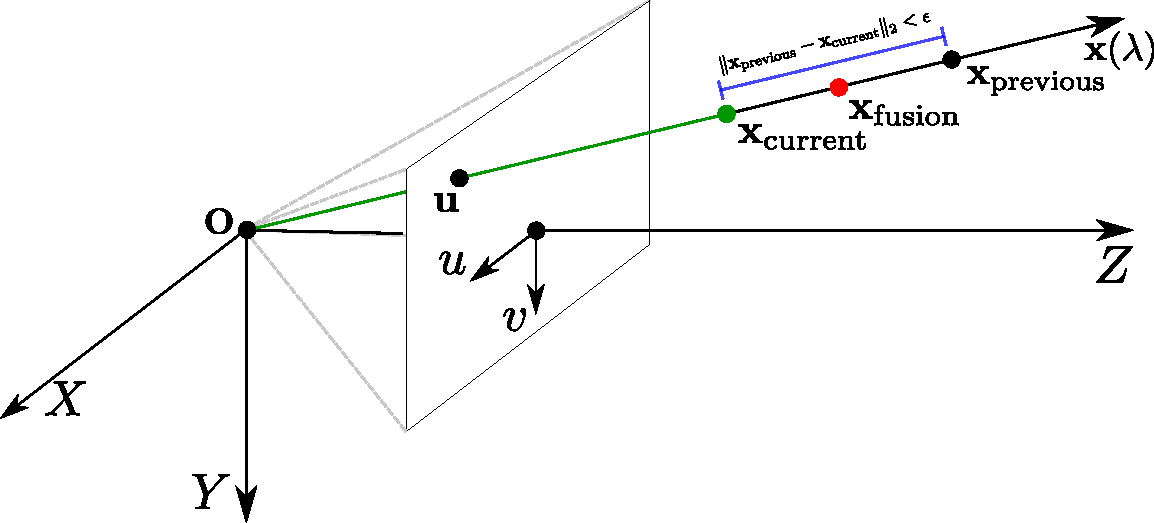
\includegraphics[width=\columnwidth]{images/map_fusion.pdf}
	\end{figure}
\end{frame}

\section{Evaluación}

\begin{frame}
	\frametitle{Datasets: KITTI y Tsukuba}
	\begin{figure}
		\subfloat[] 
		{
			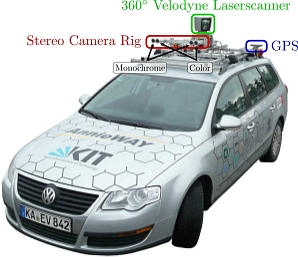
\includegraphics[width=0.3\columnwidth]{./images/kitti_sensors}
		}\hfill{}\subfloat[] 
		{
			\begin{tabular}[b]{c}%
				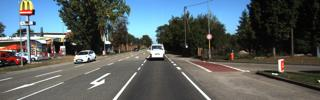
\includegraphics[width=0.3\columnwidth]{./images/kitti01}\thickspace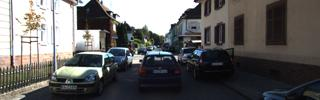
\includegraphics[width=0.3\columnwidth]{./images/kitti02}\\
				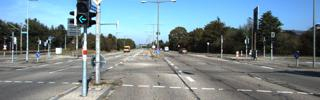
\includegraphics[width=0.3\columnwidth]{./images/kitti03}\thickspace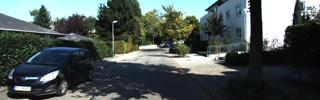
\includegraphics[width=0.3\columnwidth]{./images/kitti04}\\
				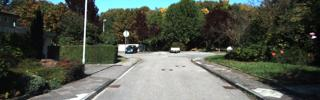
\includegraphics[width=0.3\columnwidth]{./images/kitti05}\thickspace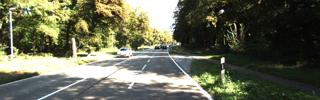
\includegraphics[width=0.3\columnwidth]{./images/kitti06}
			\end{tabular}
		}\\
		\subfloat[] 
		{
			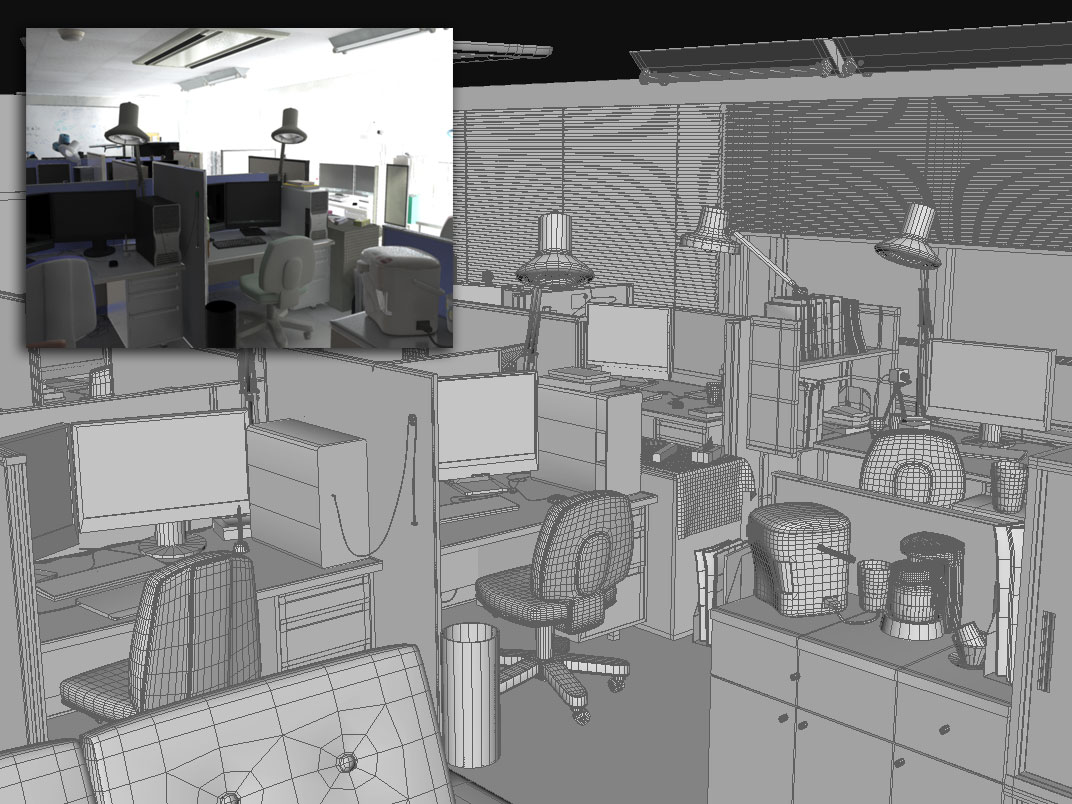
\includegraphics[width=0.3\columnwidth]{./images/tsukuba_dataset}
		}\hspace{0.2cm}\subfloat[] 
		{
			\begin{tabular}[b]{c}%
				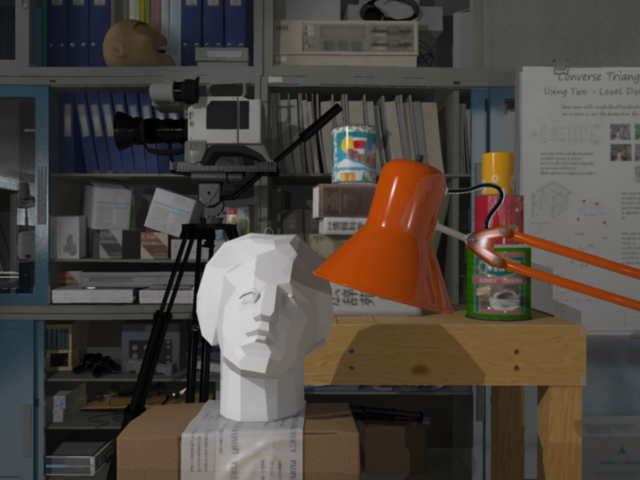
\includegraphics[width=0.2\columnwidth]{./images/tsukuba_sample1}\thickspace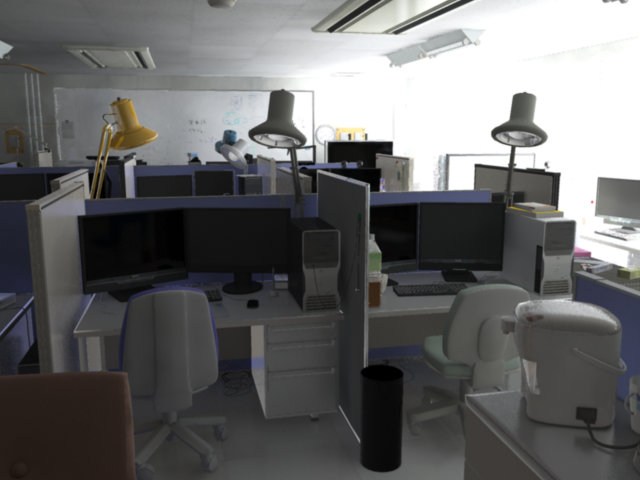
\includegraphics[width=0.2\columnwidth]{./images/tsukuba_sample2}\\
				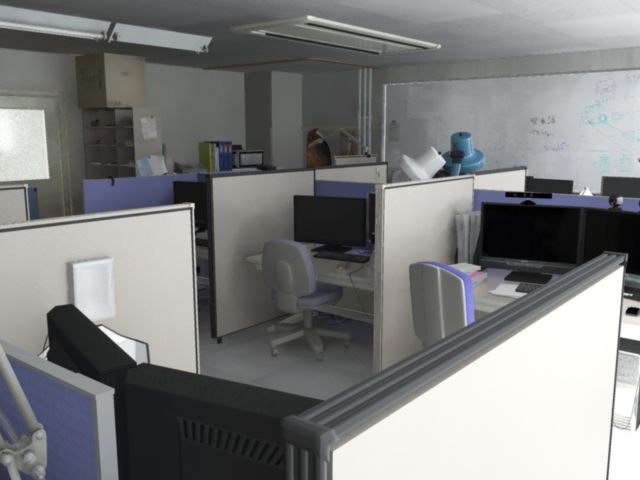
\includegraphics[width=0.2\columnwidth]{./images/tsukuba_sample3}\thickspace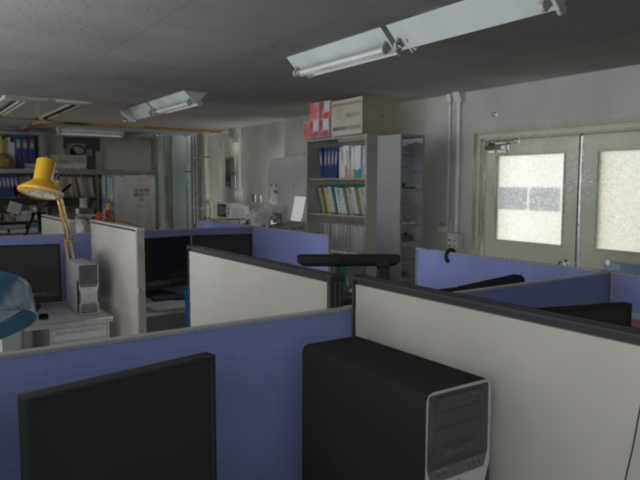
\includegraphics[width=0.2\columnwidth]{./images/tsukuba_sample4}				
			\end{tabular}
		}
	\end{figure}
\end{frame}


\begin{frame}
	\frametitle{KITTI: Reconstrucción 3D}
\begin{figure}[!htb]
	\centering
	{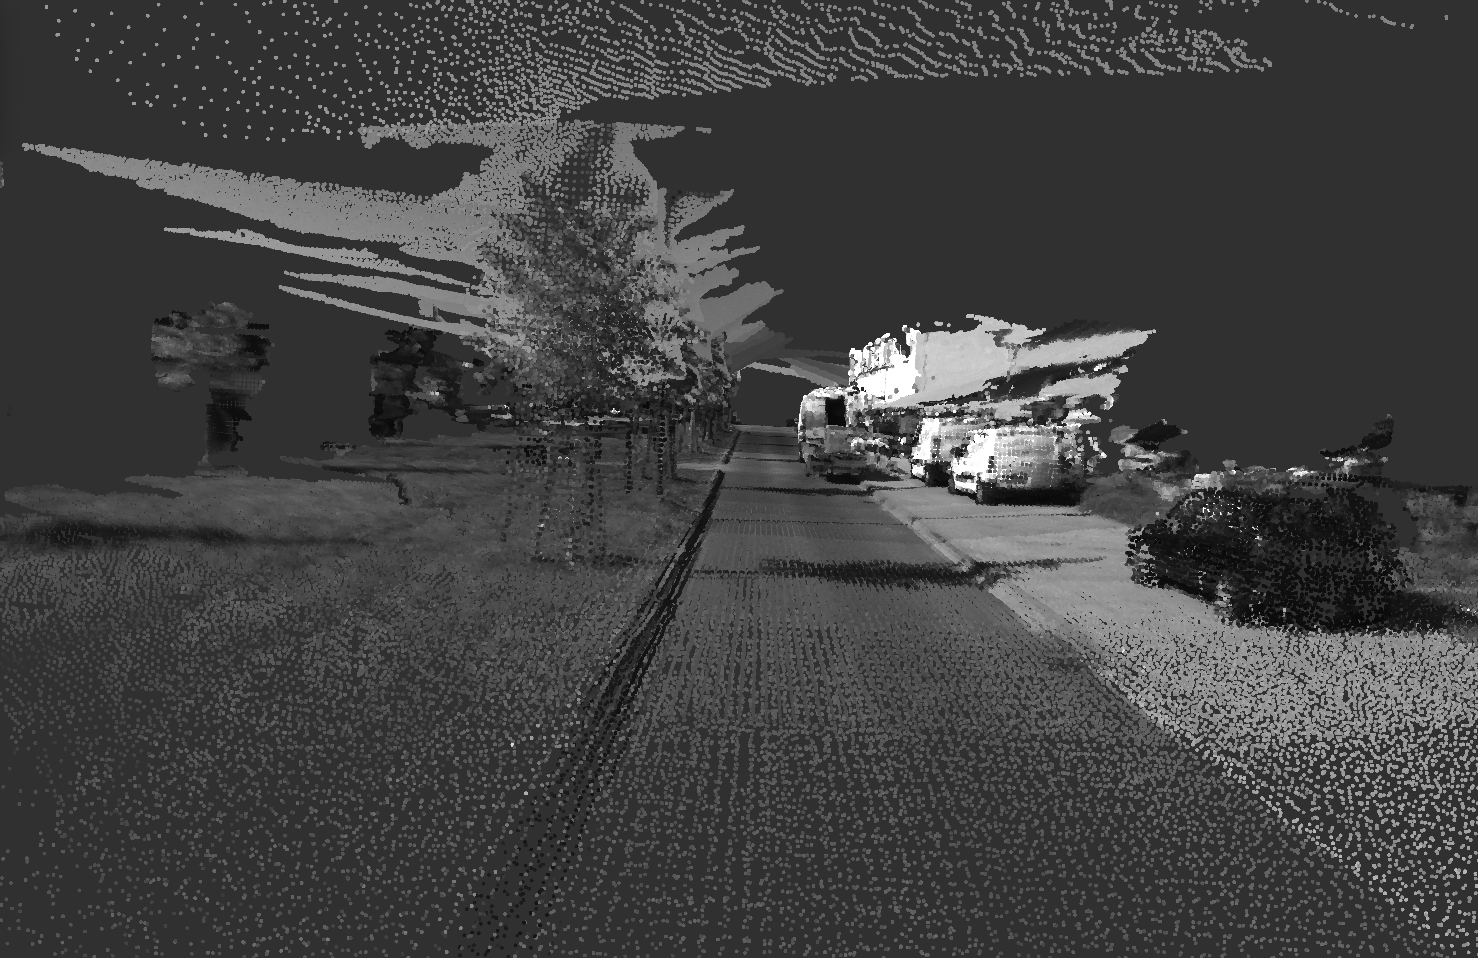
\includegraphics[width=0.32\columnwidth]{./images/kitti_3d_1}%
		\label{kitti_3d_1}}
	\hfil
	{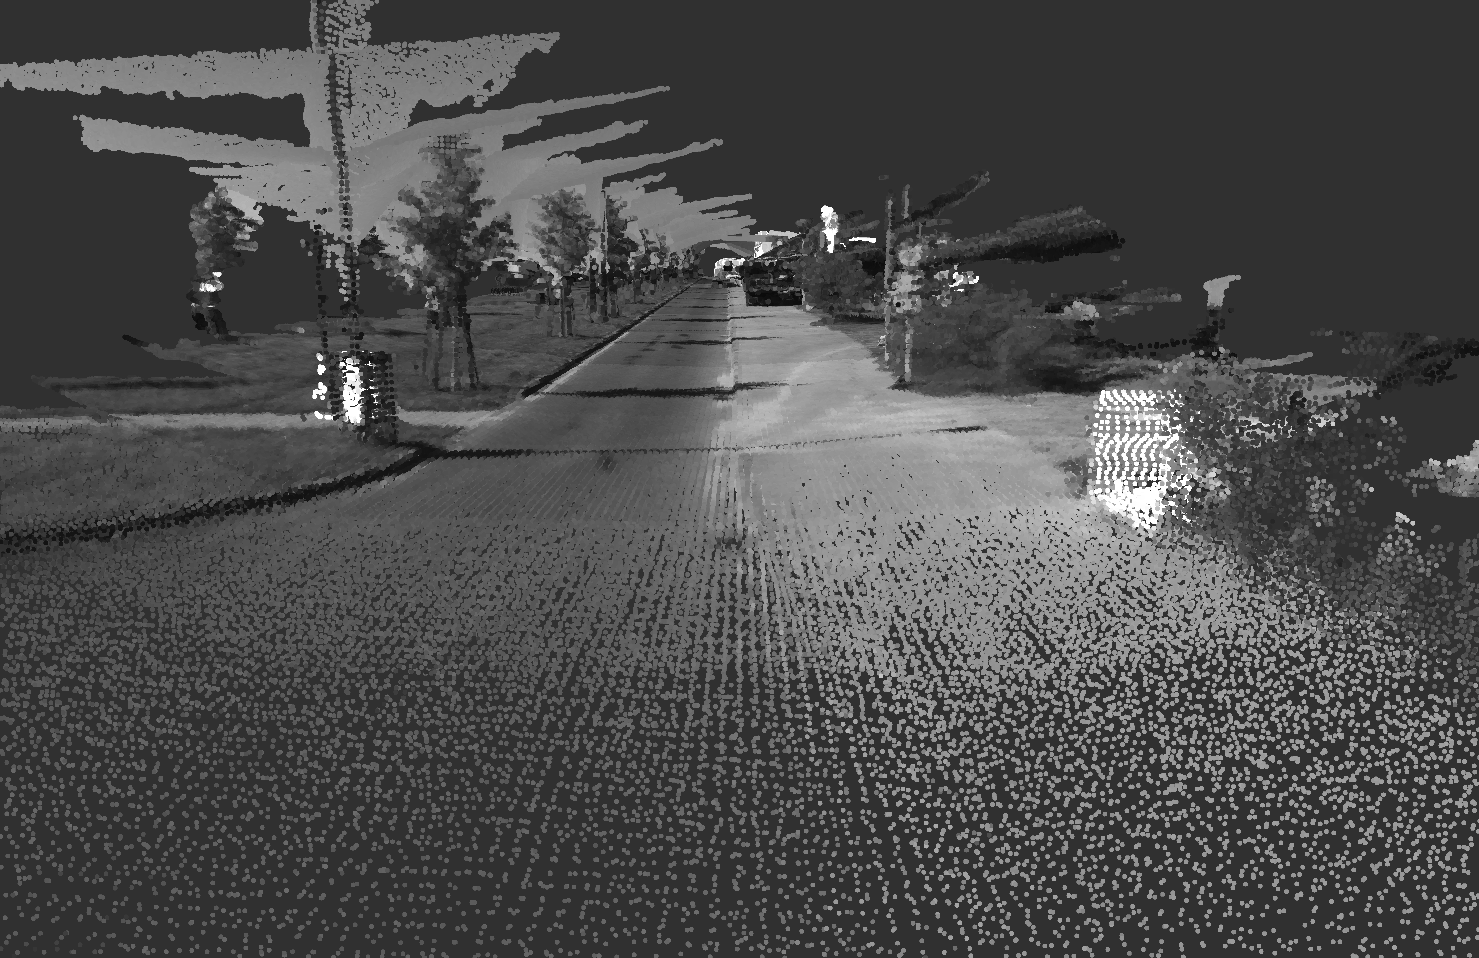
\includegraphics[width=0.32\columnwidth]{./images/kitti_3d_2}%
		\label{kitti_3d_2}}
	\hfil
	{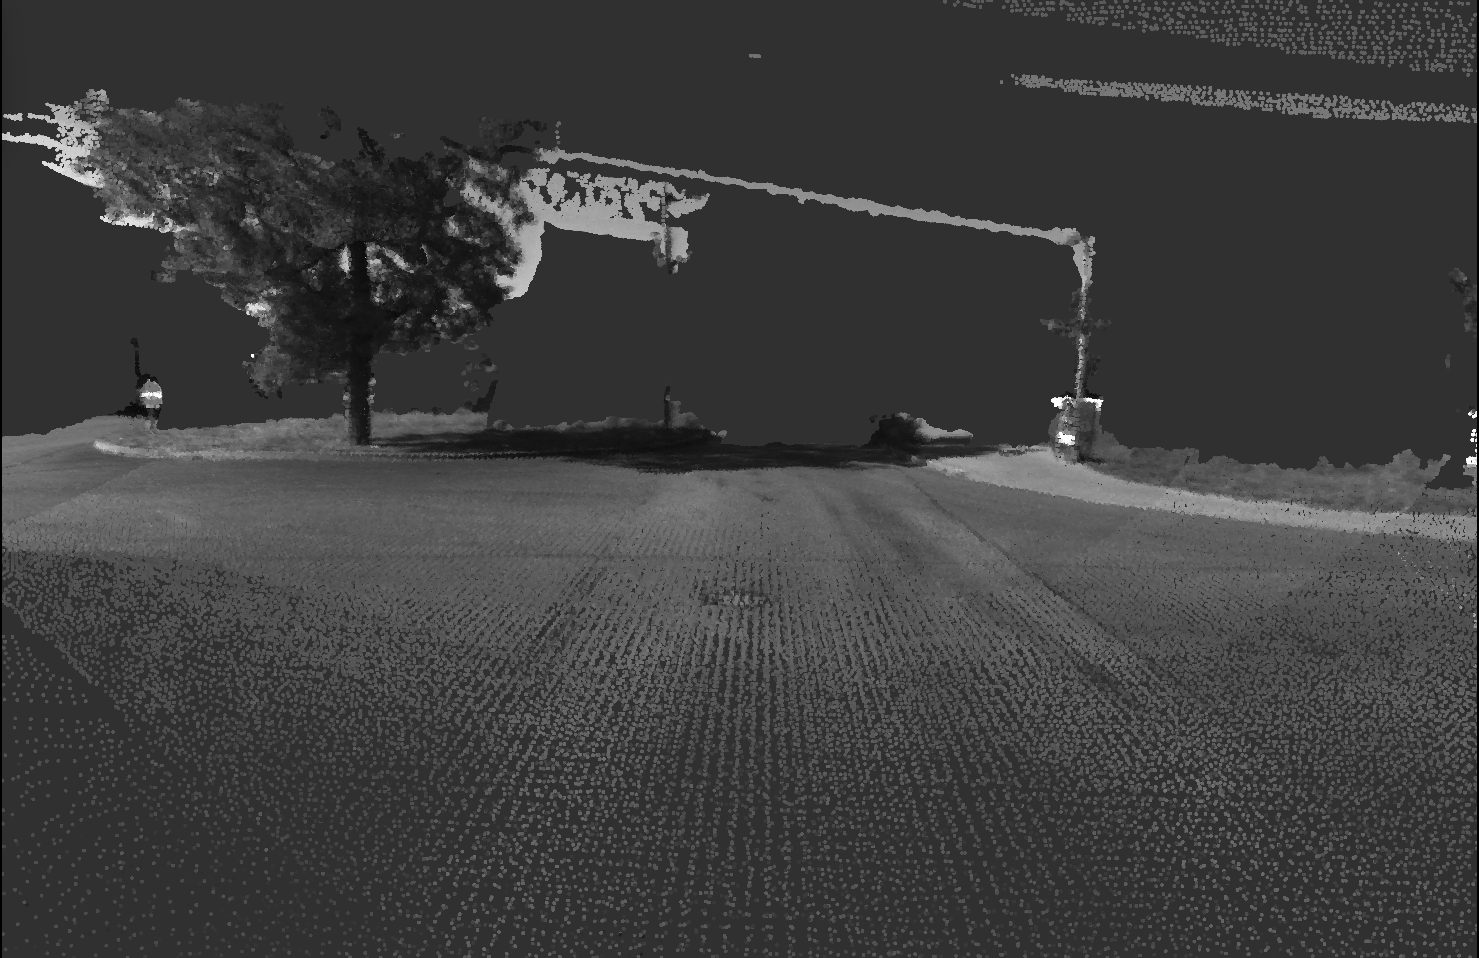
\includegraphics[width=0.32\columnwidth]{./images/kitti_3d_3}%
		\label{kitti_3d_3}}
	\\
	\caption{Several 3D reconstructions using our algorithm in the KITTI dataset (sequence 06).}
	\label{fig:kitti_reconstructions}
\end{figure}
\end{frame}

\begin{frame}
	\frametitle{Tsukuba: Reconstrucción 3D}
\begin{figure}[!htb]
	\centering
	{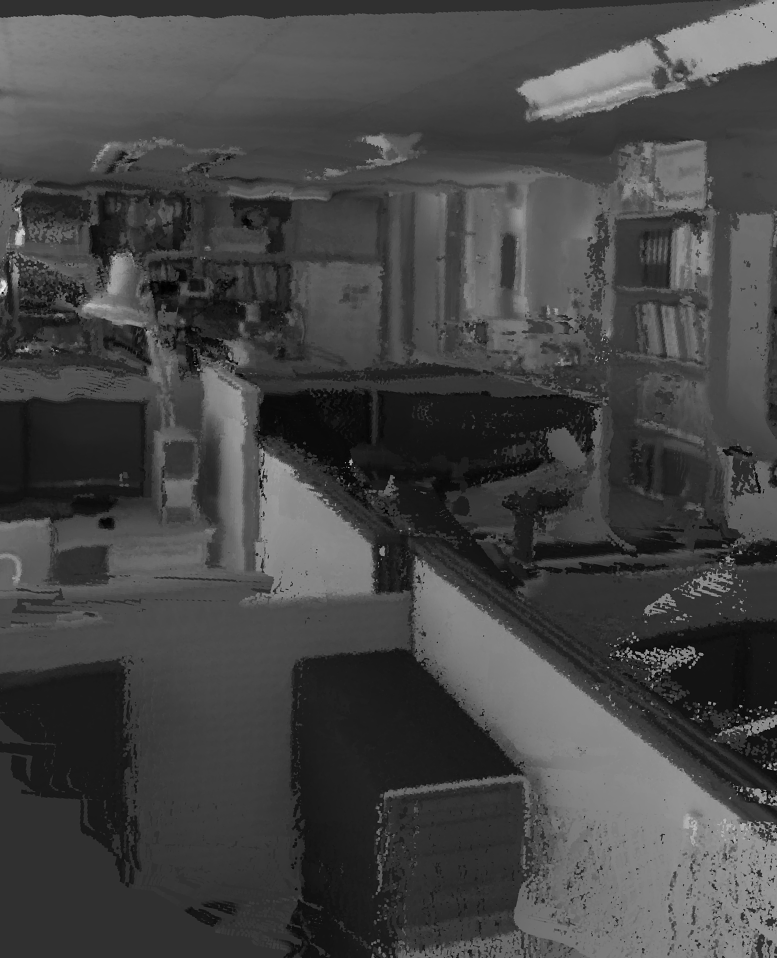
\includegraphics[width=0.32\columnwidth, height=3.5cm]{./images/tsukuba_3d_1}%
		\label{tsukuba_3d_1}}
	\hfil
	{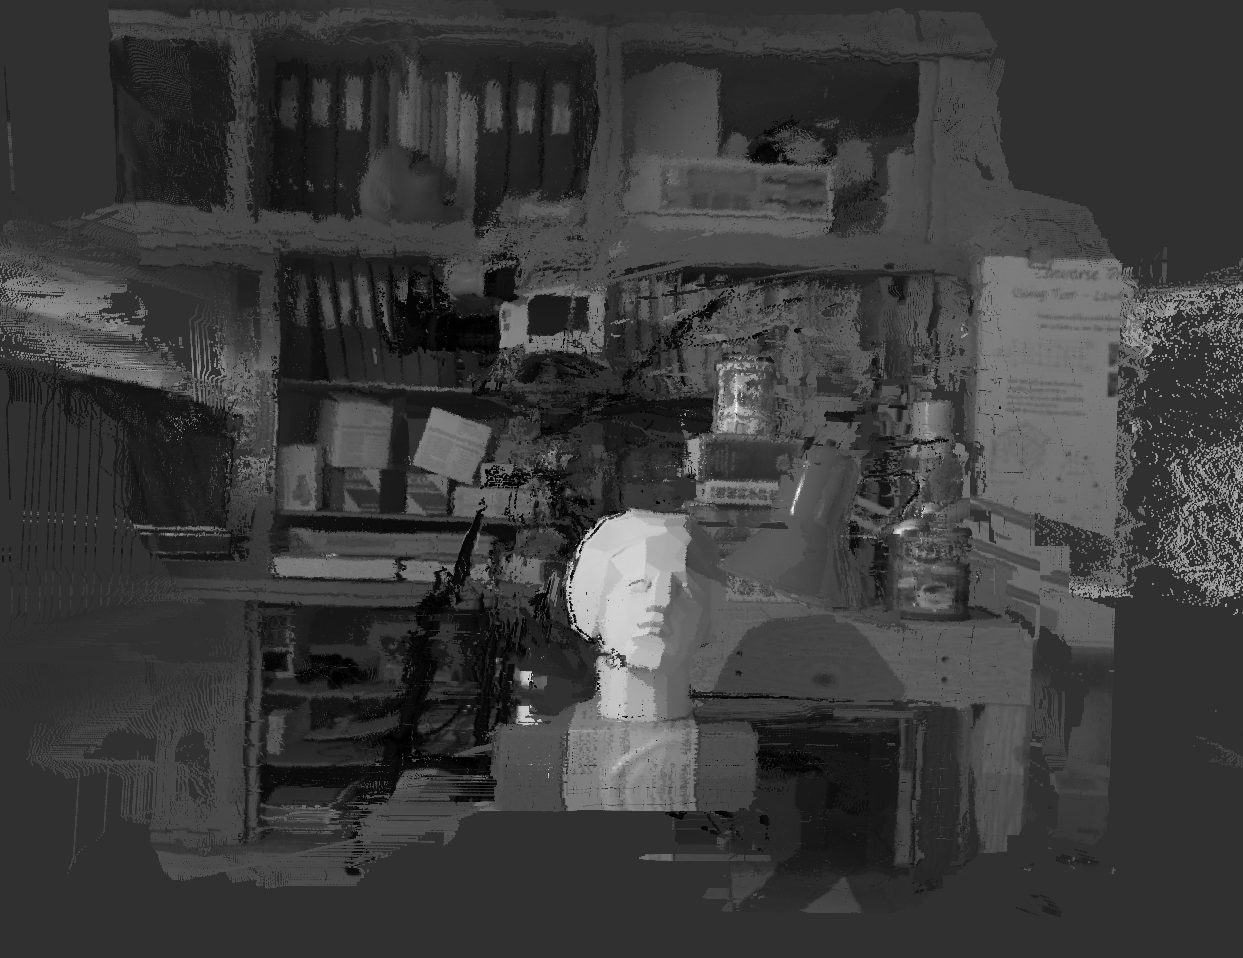
\includegraphics[width=0.32\columnwidth, height=3.5cm]{./images/tsukuba_3d_2}%
		\label{tsukuba_3d_2}}
	\hfil
	{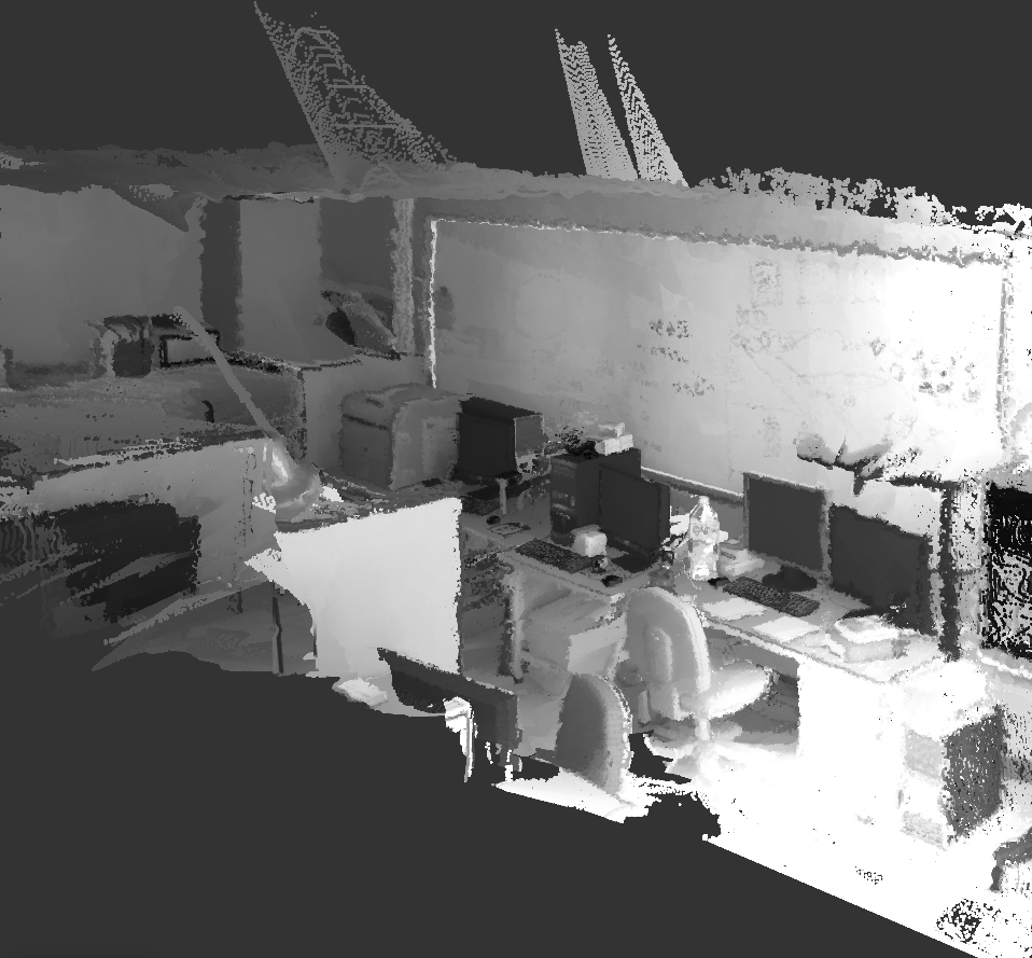
\includegraphics[width=0.32\columnwidth, height=3.5cm]{./images/tsukuba_3d_3}%
		\label{tsukuba_3d_3}}
	\hfil
	\caption{Several 3D reconstructions using our algorithm in the Tsukuba dataset.}
	\label{fig:tsukuba_reconstructions}
\end{figure}
\end{frame}

\begin{frame}
	\frametitle{KITTI: error de reconstrucción}
\begin{figure}[!htb]
	\centering
	\subfloat[Left image]{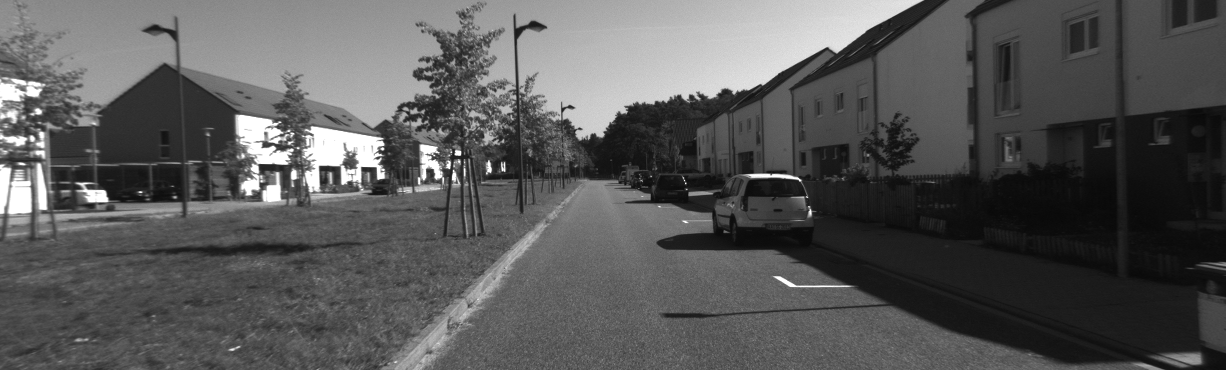
\includegraphics[width=0.45\columnwidth]{./images/kitti06_frame612_rgb.png}%
		\label{kitti06_frame612_rgb}}
	\hfil
	\subfloat[Ground-Truth]{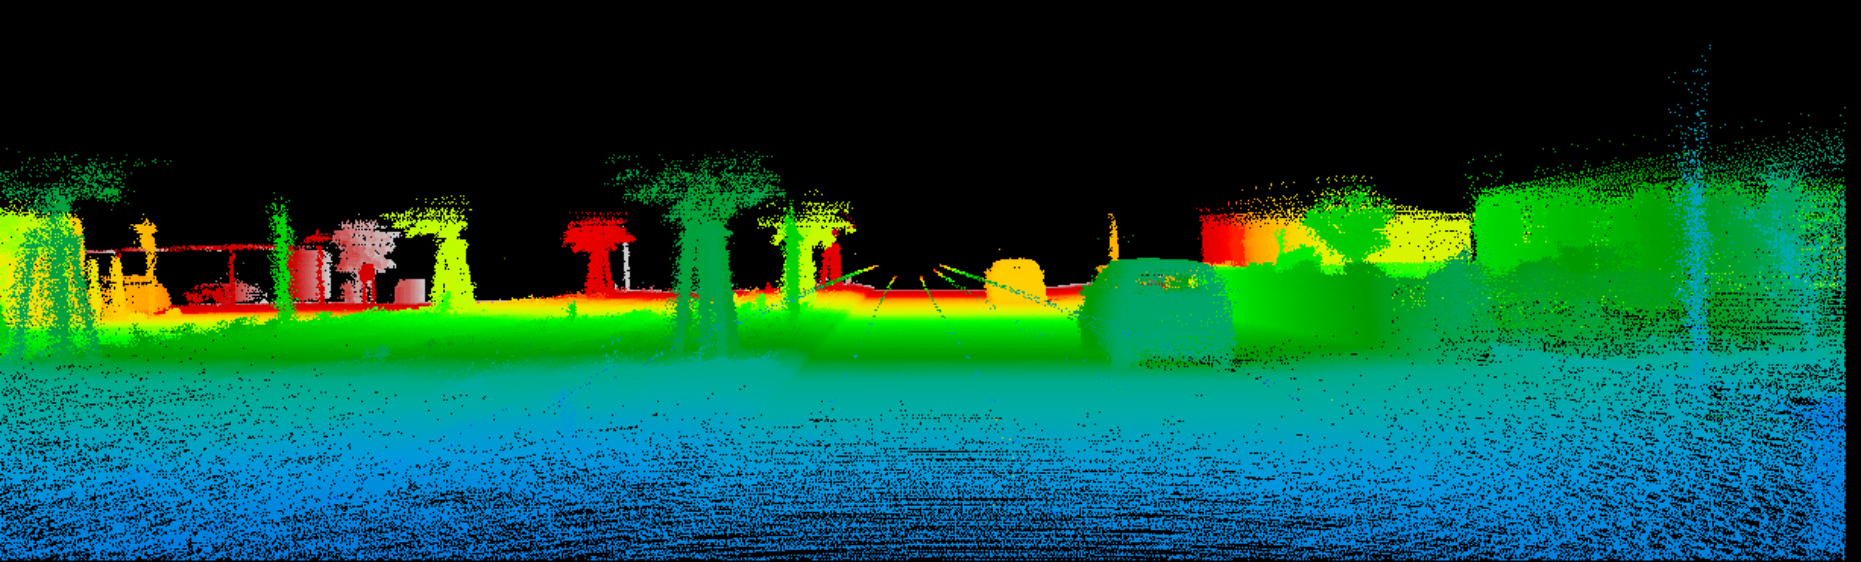
\includegraphics[width=0.45\columnwidth]{./images/kitti06_frame612_gt_high50.png}%
		\label{kitti06_frame612_gt}}
	\\
	\subfloat[LIBELAS depth map]{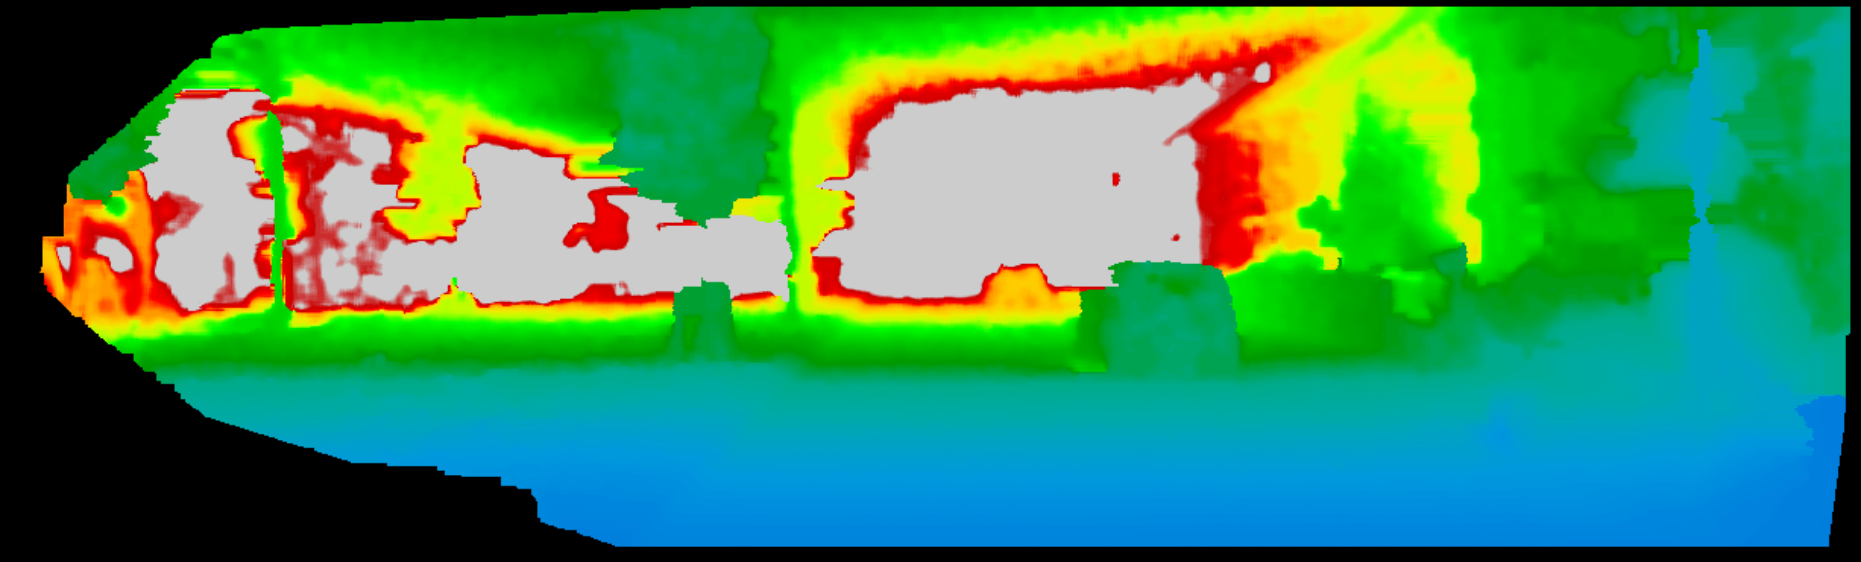
\includegraphics[width=0.45\columnwidth]{./images/kitti06_frame612_libelas_depth_high50.png}%
		\label{kitti06_frame612_libelas_depth}}
	\hfil
	\subfloat[LIBELAS depth map error]{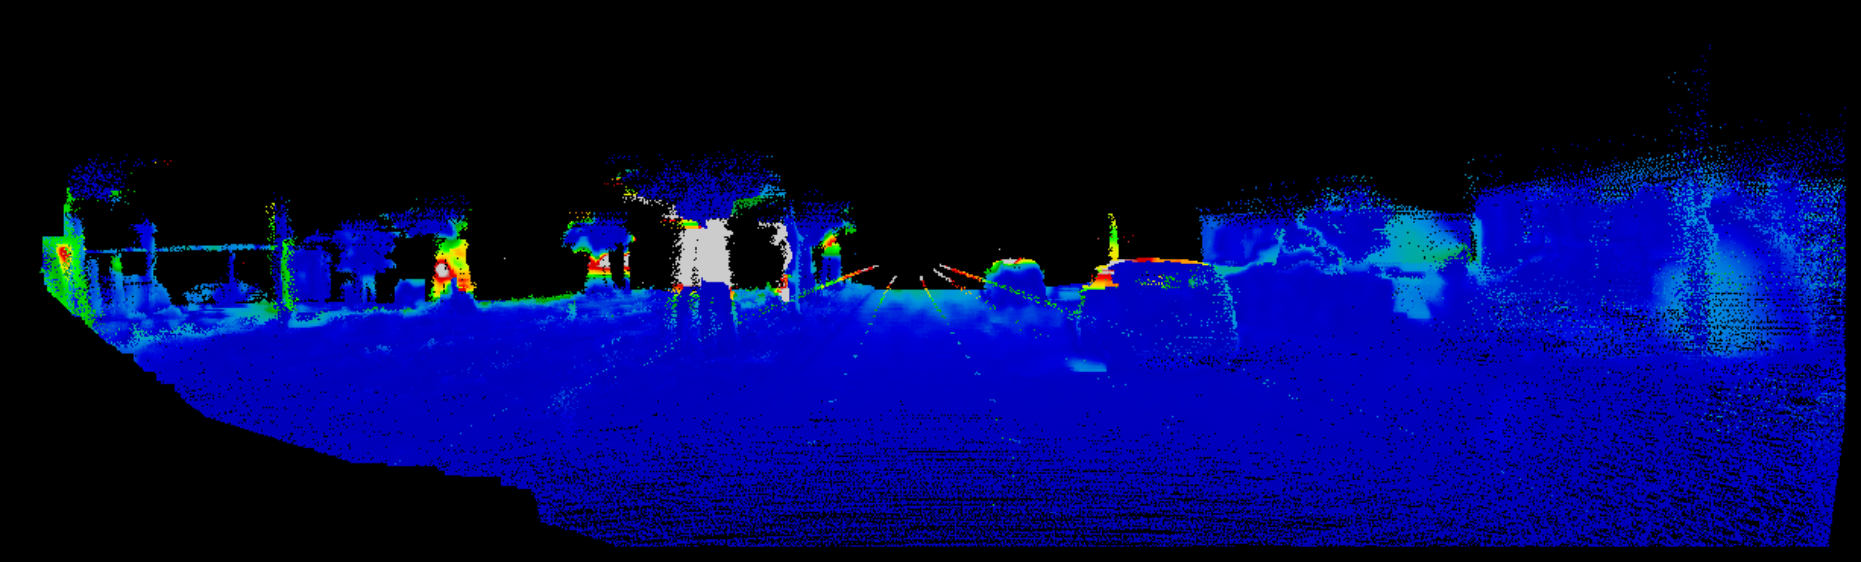
\includegraphics[width=0.45\columnwidth]{./images/kitti06_frame612_libelas_error_high50.png}%
		\label{kitti06_frame612_libelas_error}}
	\\
	\subfloat[Dense S-PTAM depth map]{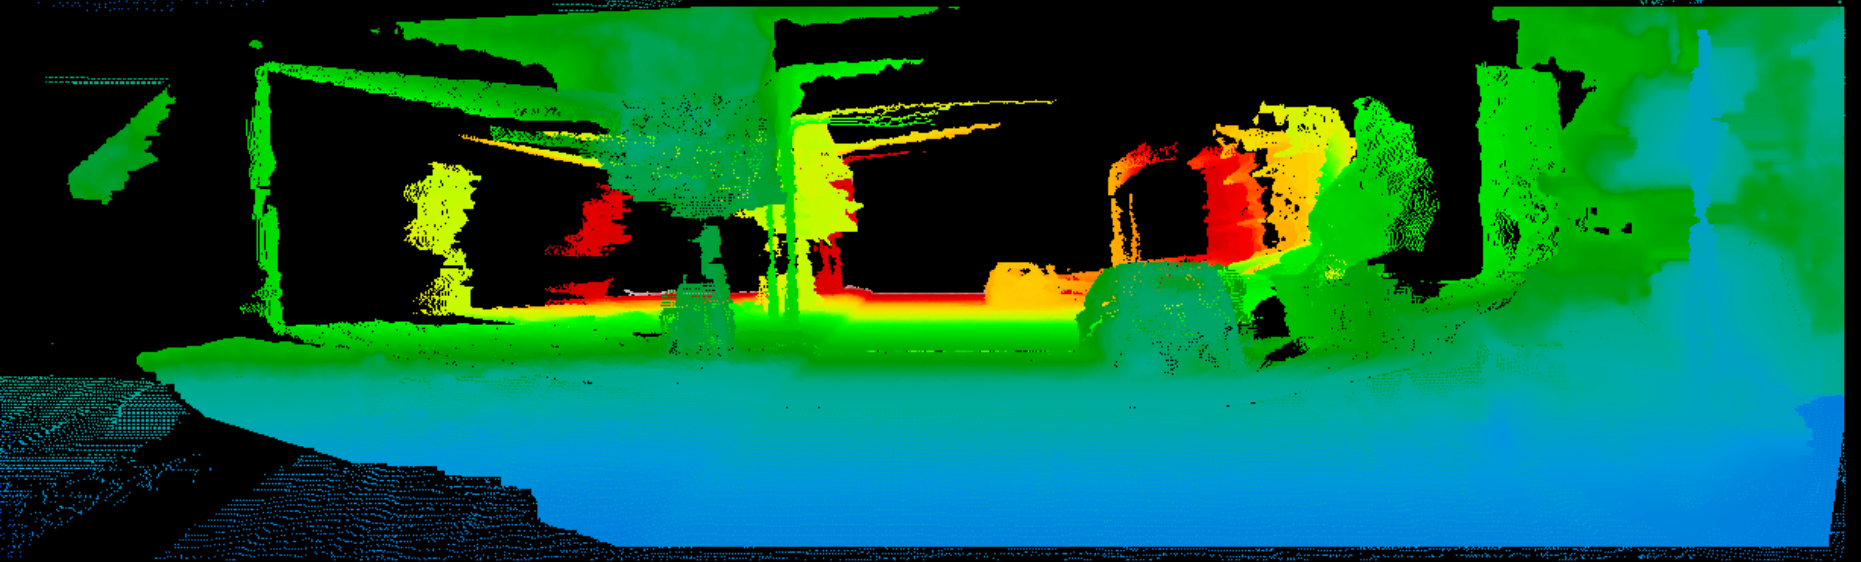
\includegraphics[width=0.45\columnwidth]{./images/kitti06_frame612_dense_high50.png}%
		\label{kitti06_frame612_dense}}
	\hfil
	\subfloat[Dense S-PTAM depth map error]{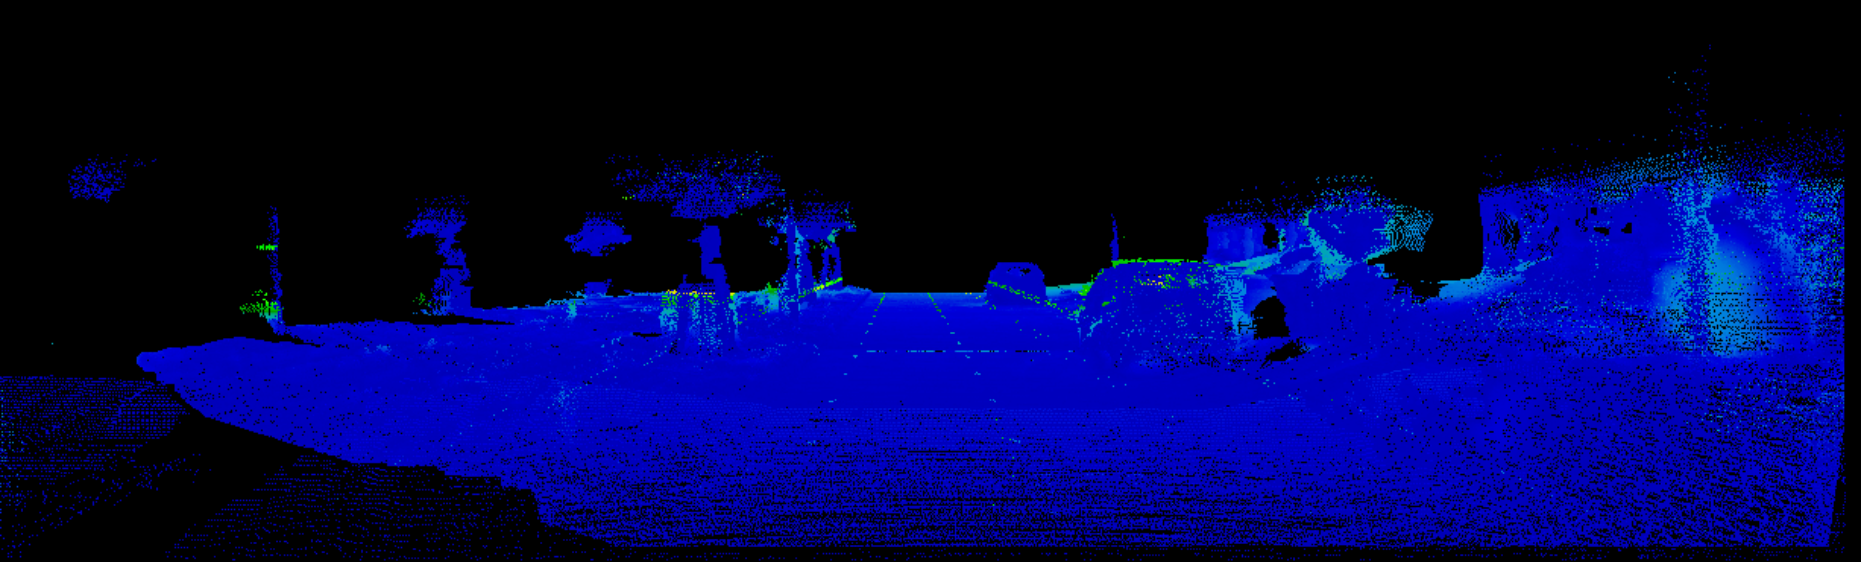
\includegraphics[width=0.45\columnwidth]{./images/kitti06_frame612_error_high50.png}%
		\label{kitti06_frame612_error}}
	\\
	\subfloat[Color metric]{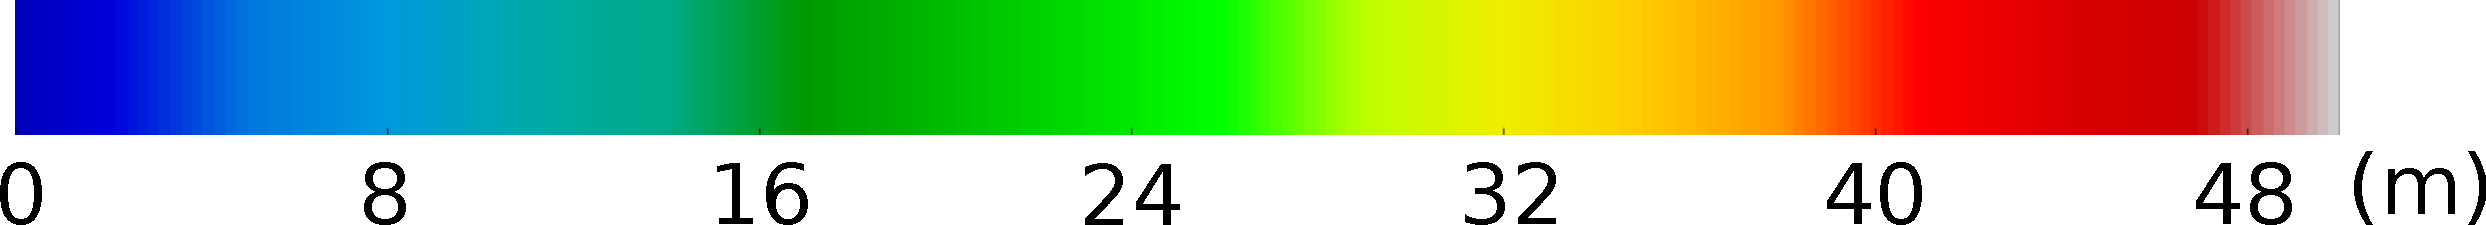
\includegraphics[width=0.45\columnwidth]{./images/high50_bar.pdf}%
		\label{kitti06_bar}}
	%\caption{Comparison of LIBELAS and Dense S-PTAM depth maps against the ground truth, for a single frame (KITTI dataset).}
	\label{fig:kitti06_frame612}
\end{figure}
\end{frame}

%\begin{frame}
%	\frametitle{KITTI: error de reconstrucción}
%\begin{figure}[!htb]
%	\centering
%	\subfloat[Left image]{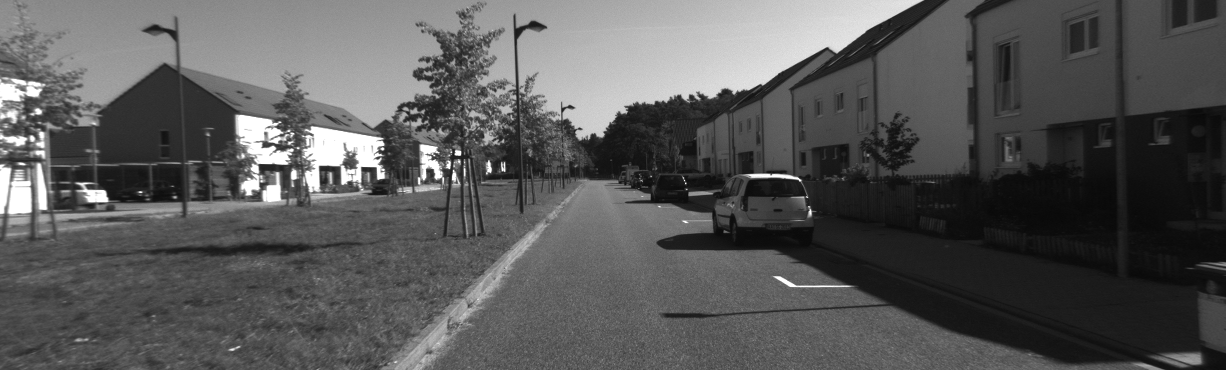
\includegraphics[width=0.45\columnwidth]{./images/kitti06_frame612_rgb.png}%
%		\label{kitti06_frame777_rgb}}
%	\hfil
%	\subfloat[Ground-Truth]{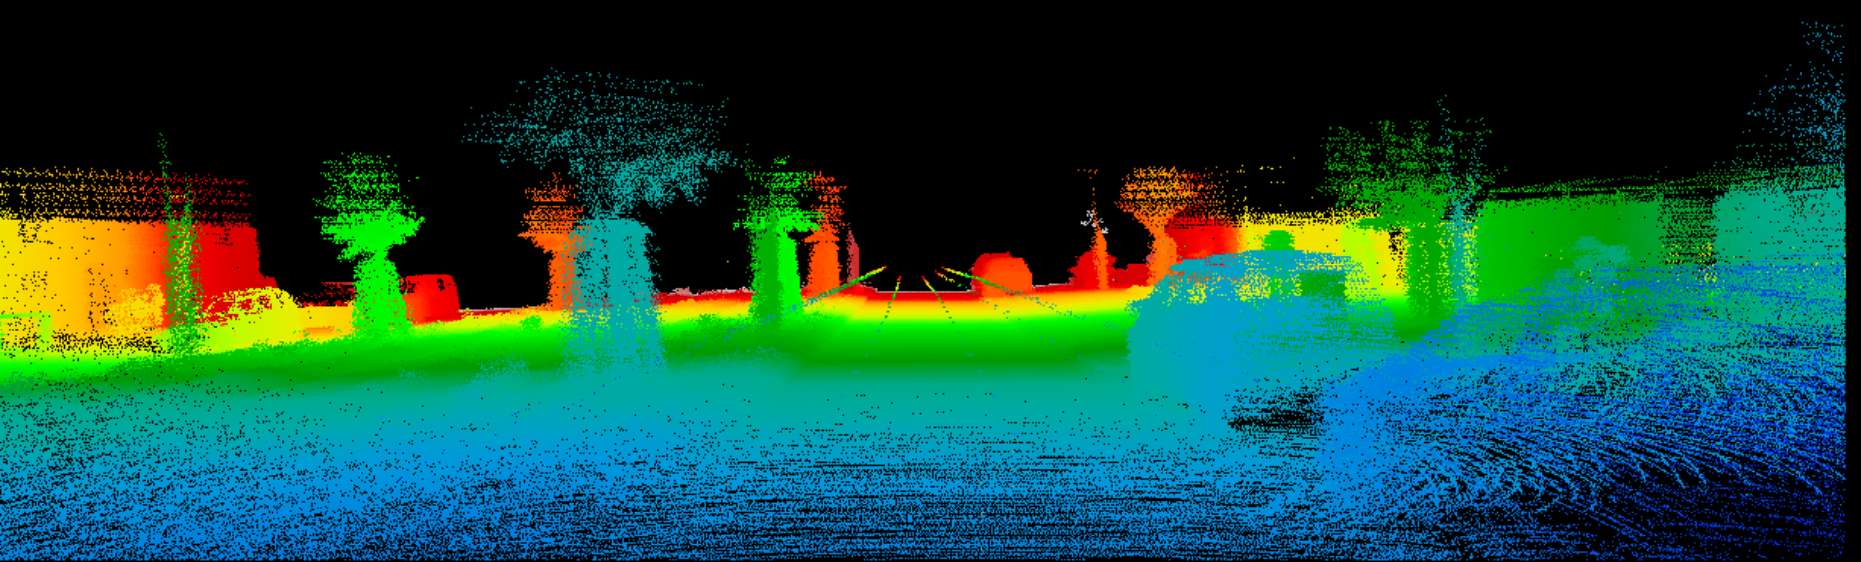
\includegraphics[width=0.45\columnwidth]{./images/kitti06_frame777_gt_high50.png}%
%		\label{kitti06_frame777_gt}}
%	\\
%	\subfloat[LIBELAS depth map]{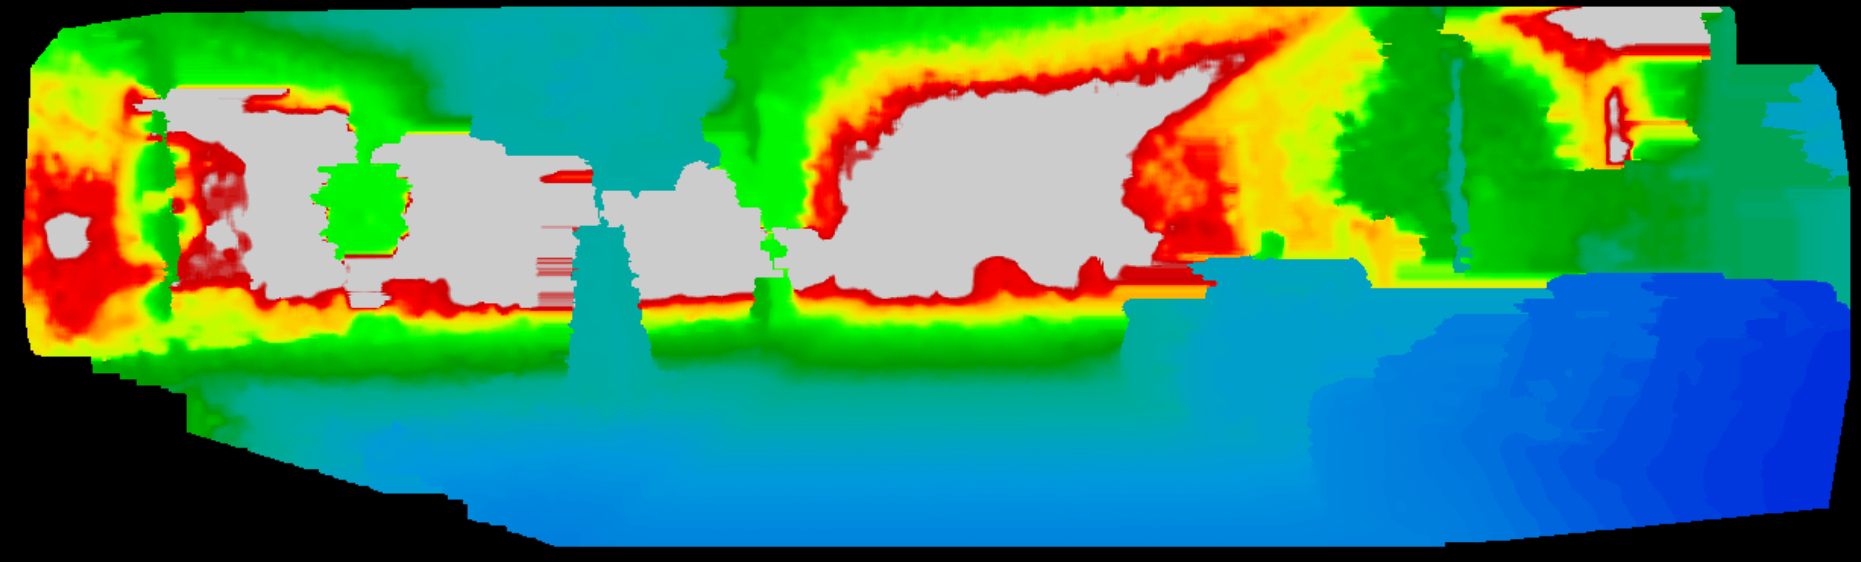
\includegraphics[width=0.45\columnwidth]{./images/kitti06_frame777_libelas_depth_high50.png}%
%		\label{kitti06_frame777_libelas_depth}}
%	\hfil
%	\subfloat[LIBELAS Depth map error]{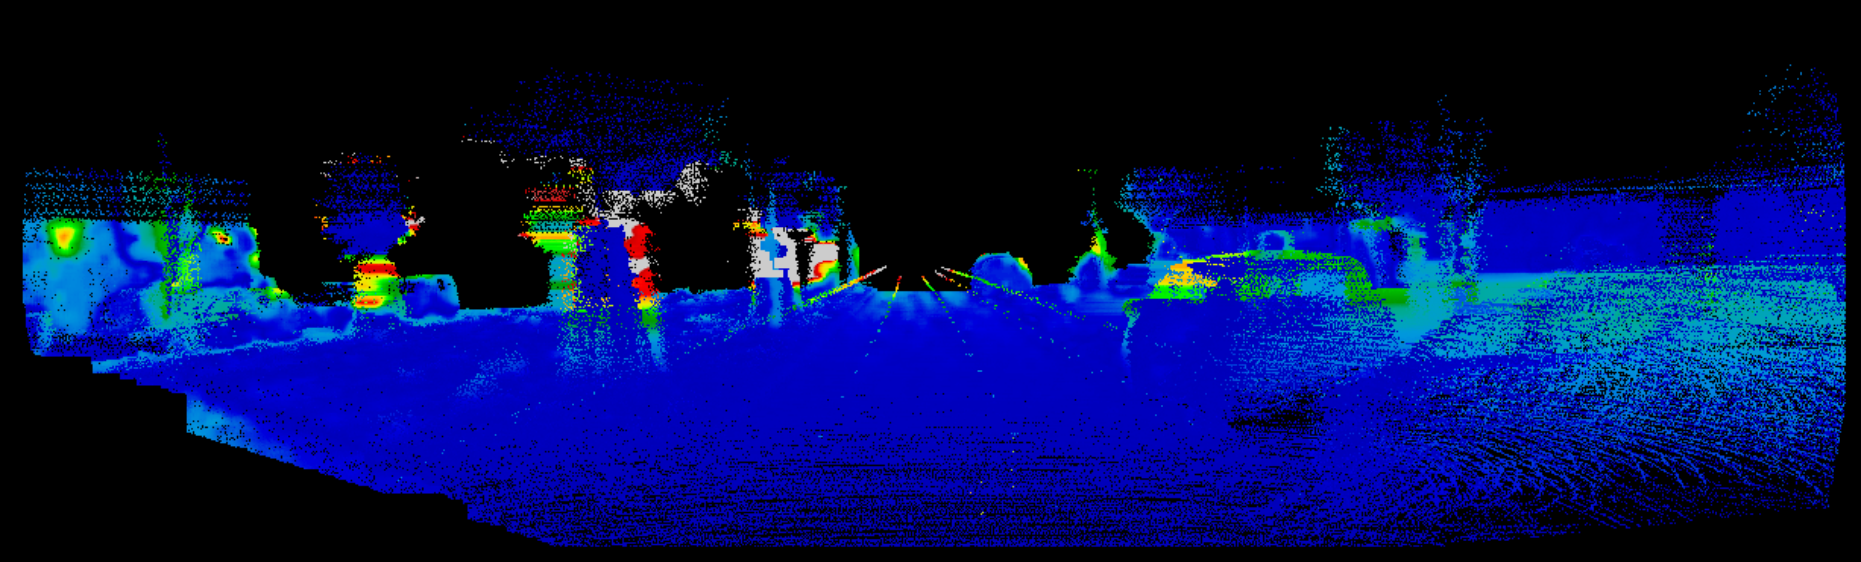
\includegraphics[width=0.45\columnwidth]{./images/kitti06_frame777_libelas_error_high50.png}%
%		\label{kitti06_frame777_libelas_error}}
%	\\
%	\subfloat[Dense S-PTAM depth map]{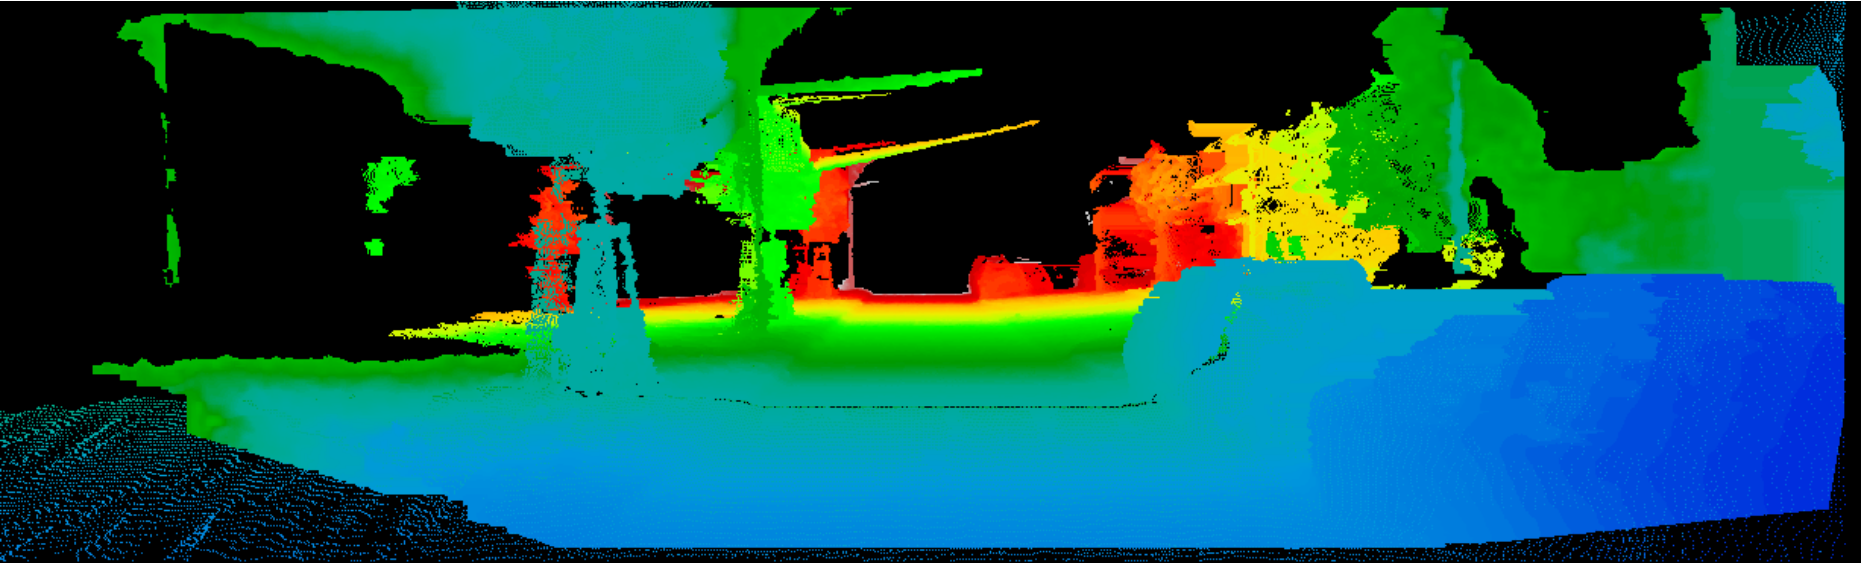
\includegraphics[width=0.45\columnwidth]{./images/kitti06_frame777_dense_high50.png}%
%		\label{kitti06_frame777_dense}}
%	\hfil
%	\subfloat[Dense S-PTAM depth map error]{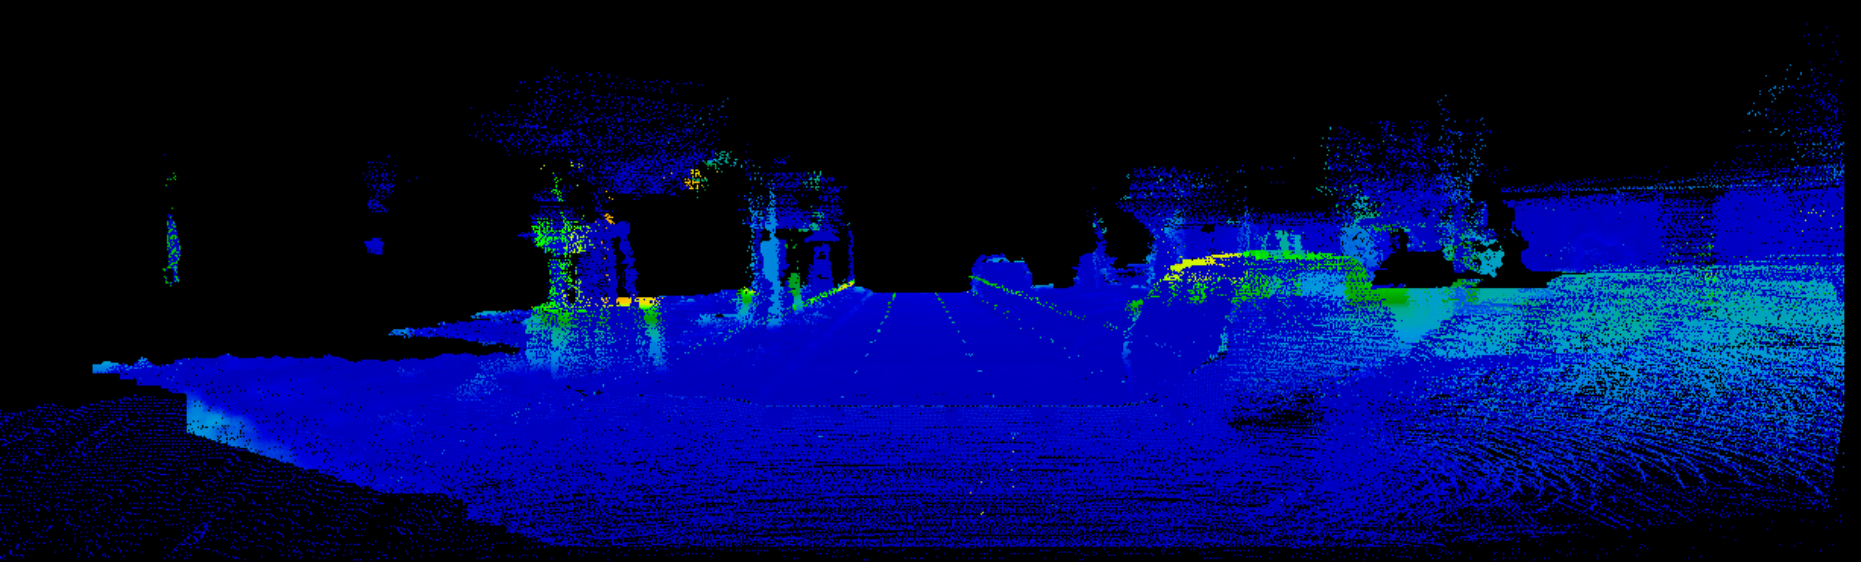
\includegraphics[width=0.45\columnwidth]{./images/kitti06_frame777_error_high50.png}%
%		\label{kitti06_frame777_error}}
%	\\
%	\subfloat[Color metric]{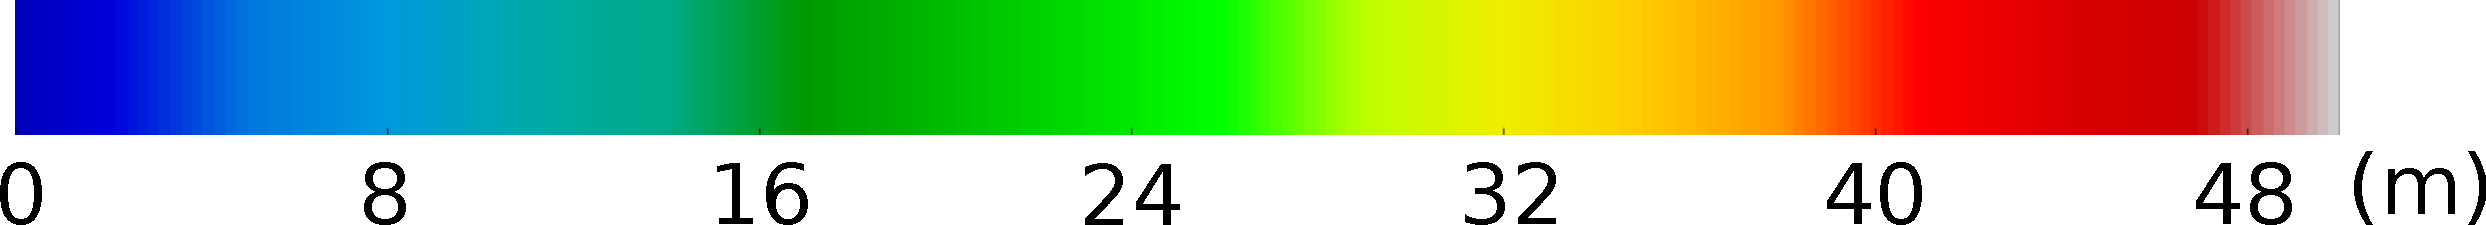
\includegraphics[width=0.45\columnwidth]{./images/high50_bar.pdf}%
%		\label{kitti06_frame777_bar}}
%	\caption{Comparison of LIBELAS and Dense S-PTAM depth maps against the ground truth, for a single frame (KITTI dataset).}
%	\label{fig:kitti06_frame777}
%\end{figure}
%\end{frame}


\begin{frame}
	\frametitle{Tsukuba: error de reconstrucción}
% tsukuba
\begin{figure}[!htb]
	\centering
	\subfloat[Left image]{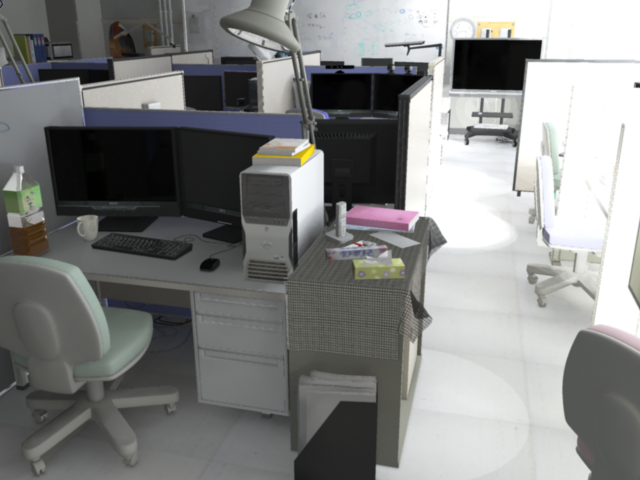
\includegraphics[width=0.2\columnwidth]{./images/tsukuba_frame807_rgb.png}%
		\label{tsukuba_frame807_rgb}}
	\hfil
	\subfloat[Ground Truth]{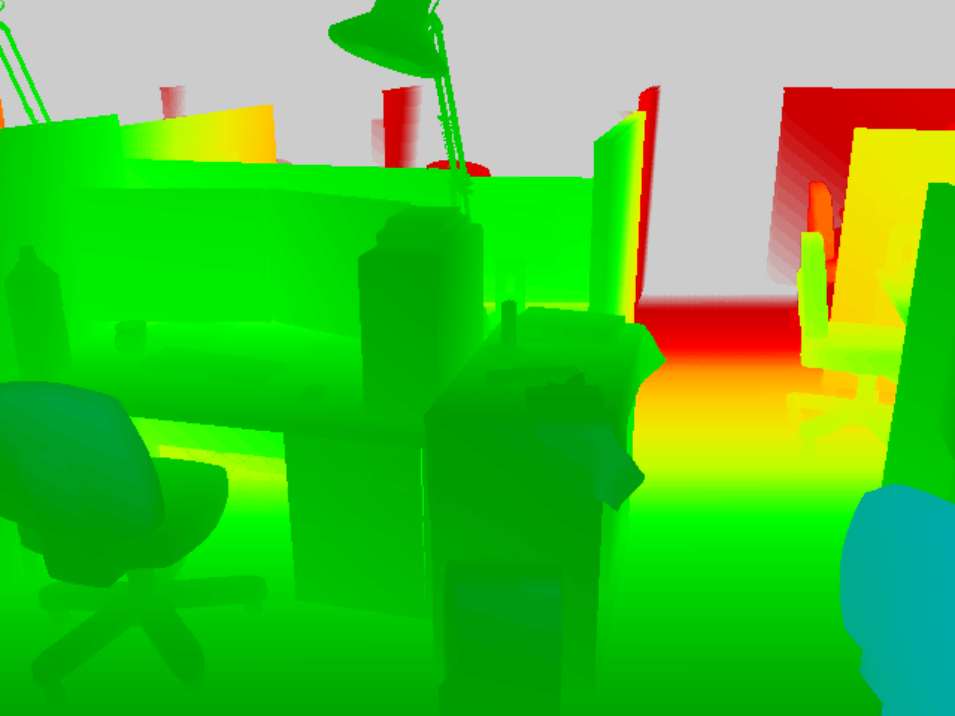
\includegraphics[width=0.2\columnwidth]{./images/tsukuba_frame807_gt_high6.png}%
		\label{tsukuba_gt}}
    \\
	\subfloat[LIBELAS dmap]{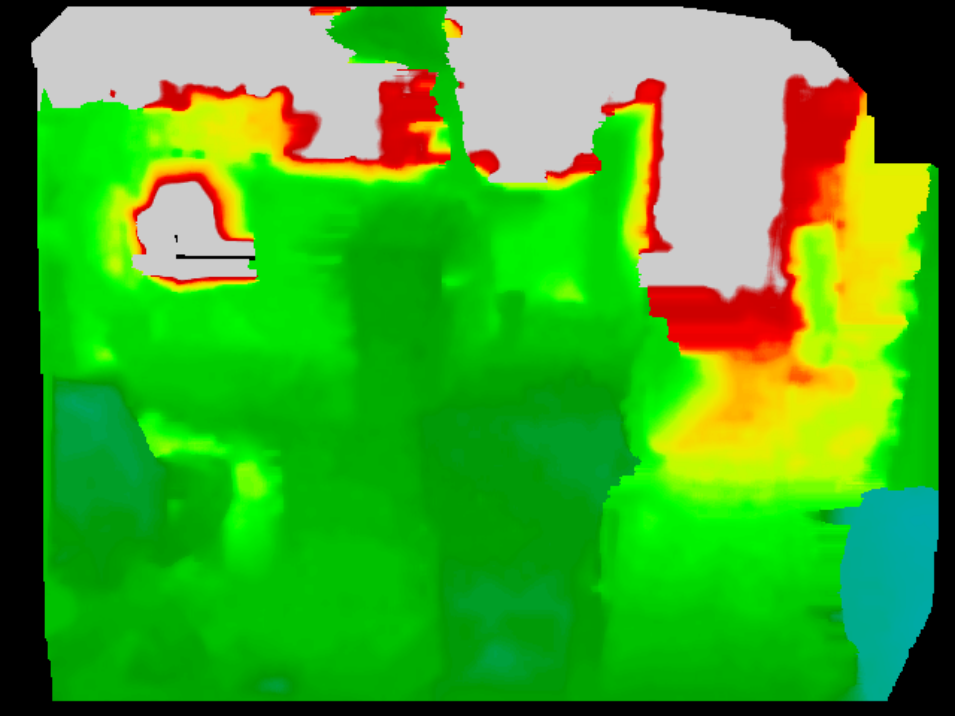
\includegraphics[width=0.2\columnwidth]{./images/tsukuba_frame807_libelas_depth_high6.png}%
		\label{tsukuba_frame807_libelas_depth}}
	\hfil
	\subfloat[LIBELAS dmap error]{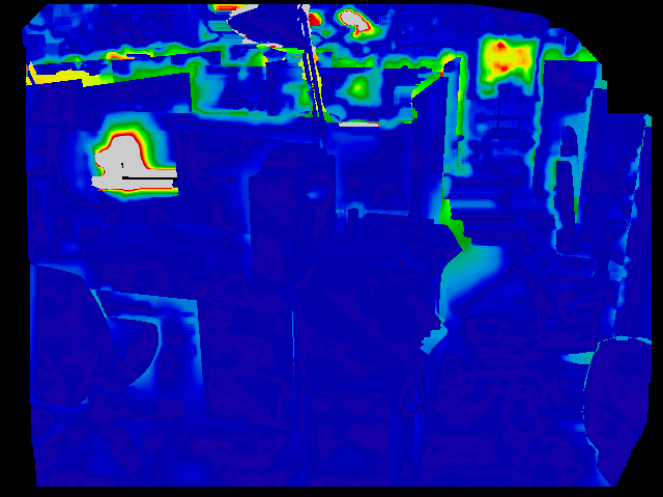
\includegraphics[width=0.2\columnwidth]{./images/tsukuba_frame807_libelas_error_high6.png}%
		\label{tsukuba_frame807_libelas_error}}
    \hfil
	\subfloat[Dense S-PTAM dmap]{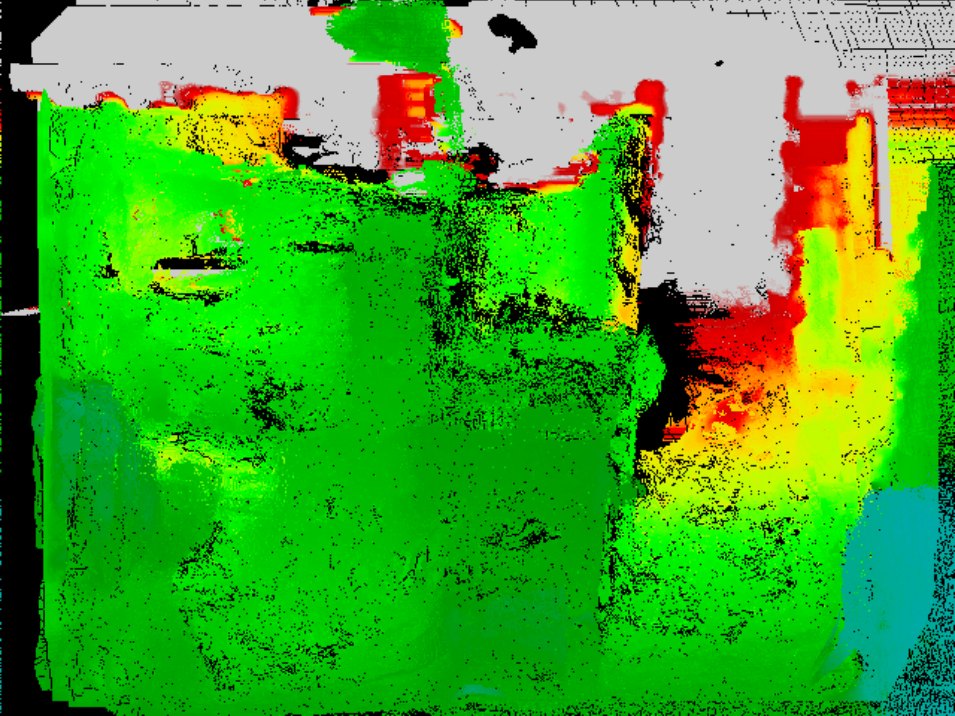
\includegraphics[width=0.2\columnwidth]{./images/tsukuba_frame807_dense_high6.png}%
		\label{tsukuba_frame807_dense}}
	\hfil
	\subfloat[Dense S-PTAM dmap error]{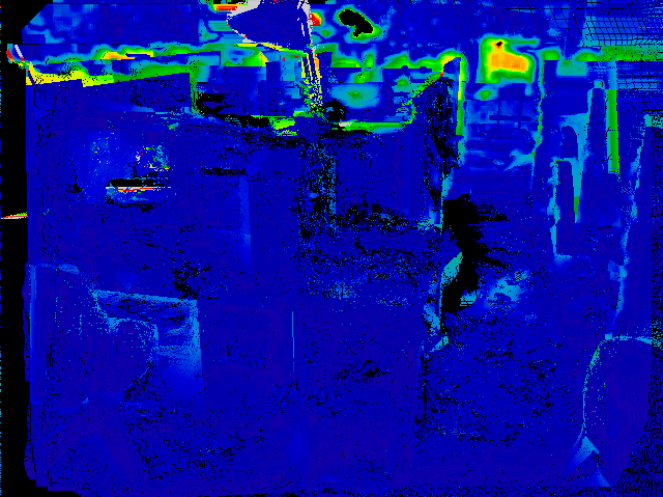
\includegraphics[width=0.2\columnwidth]{./images/tsukuba_frame807_error_high6.png}%
		\label{tsukuba_frame807_error}}
	\\
	\subfloat[]{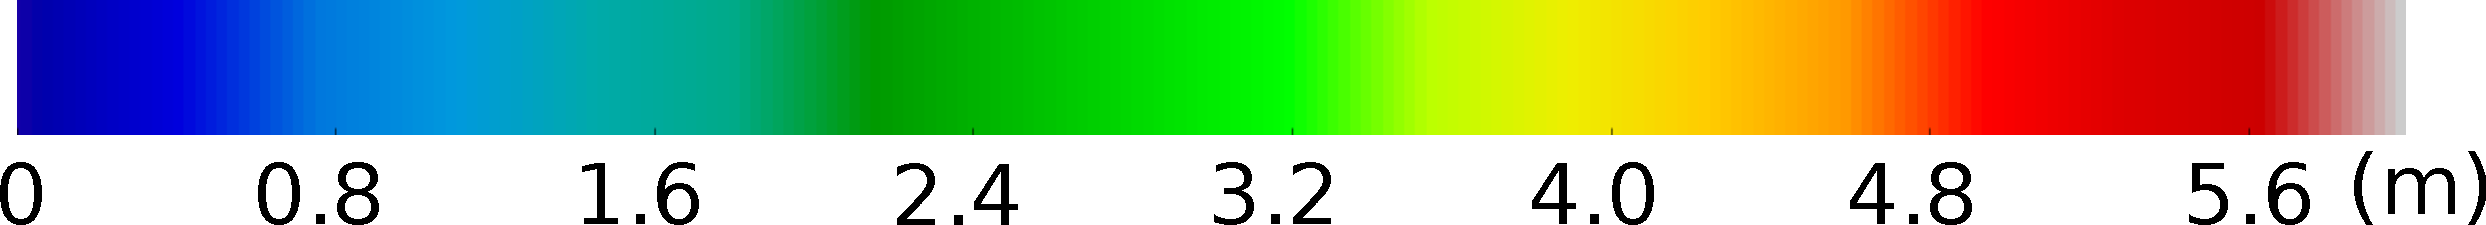
\includegraphics[width=0.4\columnwidth]{./images/high6_bar.pdf}%
		\label{tsukuba_frame807_bar}}
	%\caption{Comparison: LIBELAS, DS-PTAM dmaps against GT (Tsukuba).}
	\label{fig:tsukuba_frame807}
\end{figure}
\end{frame}

%\begin{frame}
%	\frametitle{Tsukuba: error de reconstrucción}
%	\begin{figure}[!htb]
%		\centering
%		\subfloat[Left image]{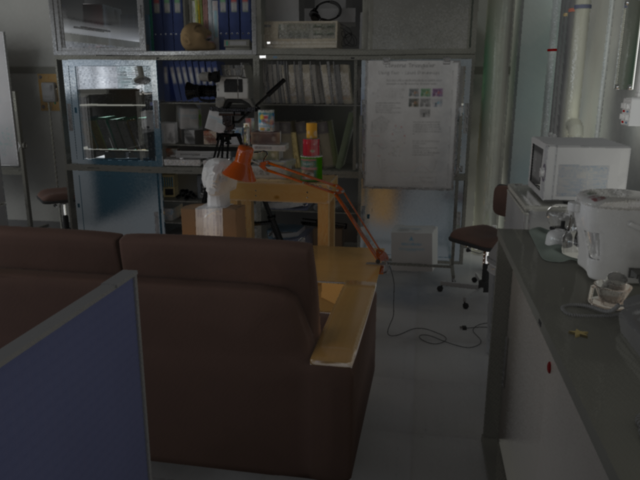
\includegraphics[width=0.2\columnwidth]{./images/tsukuba_frame1314_rgb.png}%
%			\label{tsukuba_frame1314_rgb}}
%        \hfil
%		\subfloat[Ground Truth]{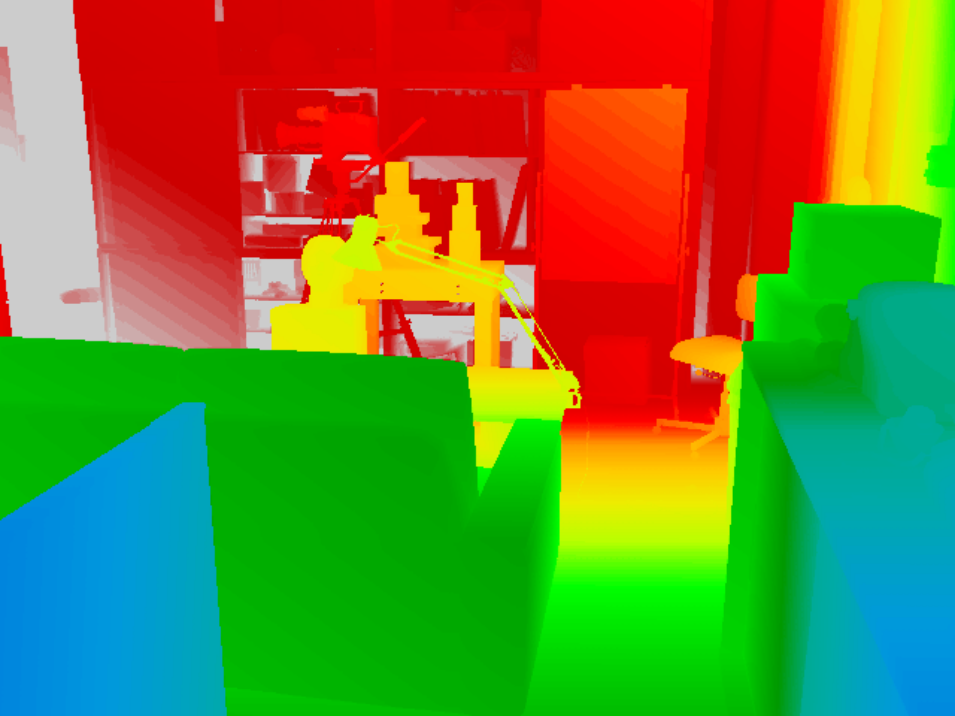
\includegraphics[width=0.2\columnwidth]{./images/tsukuba_frame1314_gt_high6.png}%
%			\label{tsukuba_frame1314_gt}}
%        \\
%		\subfloat[LIBELAS dmap]{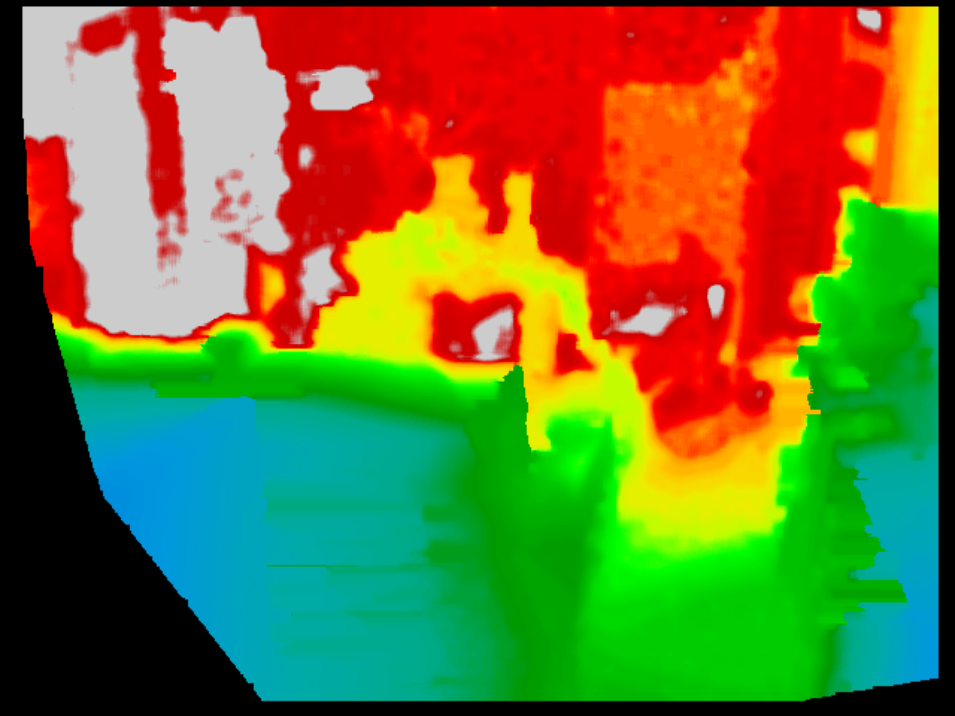
\includegraphics[width=0.2\columnwidth]{./images/tsukuba_frame1314_libelas_depth_high6.png}%
%			\label{tsukuba_frame1314_libelas_depth}}
%        \hfil
%		\subfloat[LIBELAS dmap error]{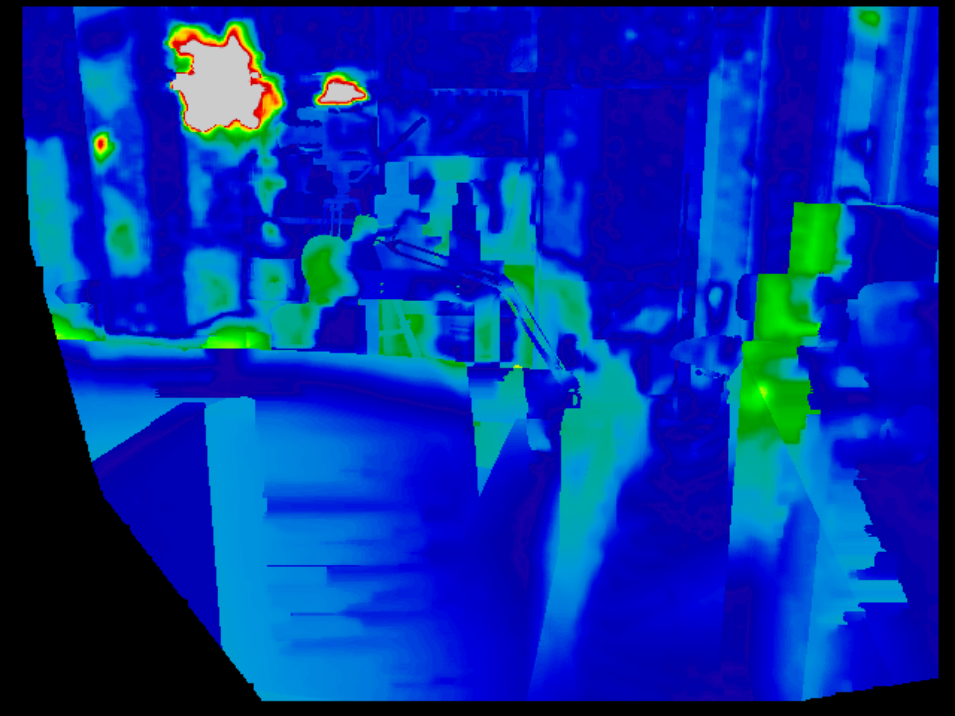
\includegraphics[width=0.2\columnwidth]{./images/tsukuba_frame1314_libelas_error_high6.png}%
%			\label{tsukuba_frame1314_libelas_error}}
%        \hfil
%		\subfloat[Dense S-PTAM dmap]{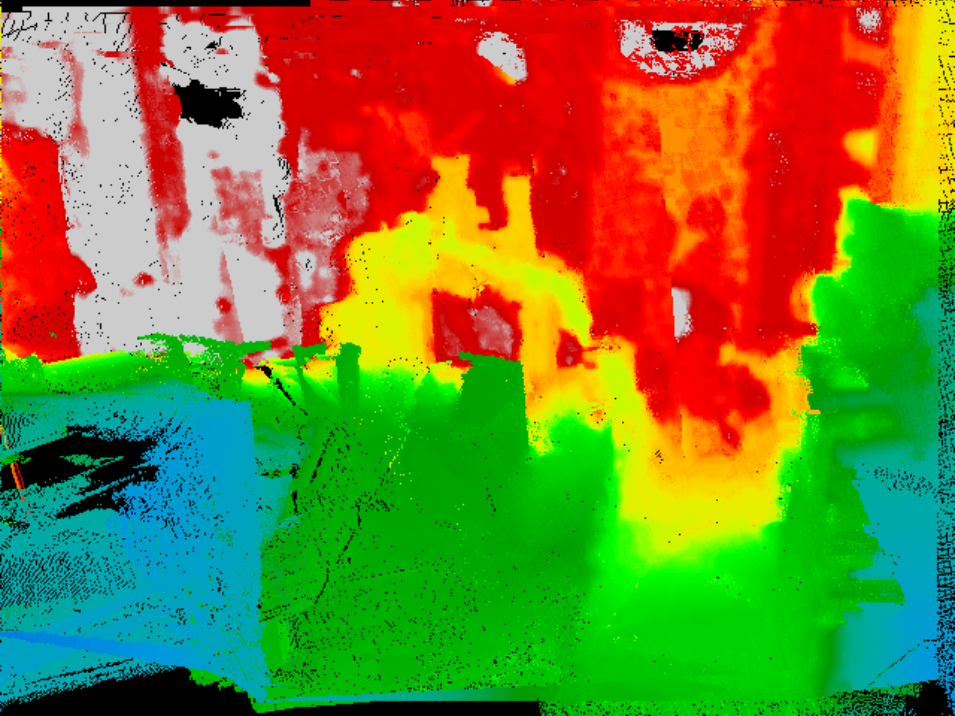
\includegraphics[width=0.2\columnwidth]{./images/tsukuba_frame1314_dense_high6.png}%
%			\label{tsukuba_frame1314_dense}}
%        \hfil
%		\subfloat[Dense S-PTAM dmap error]{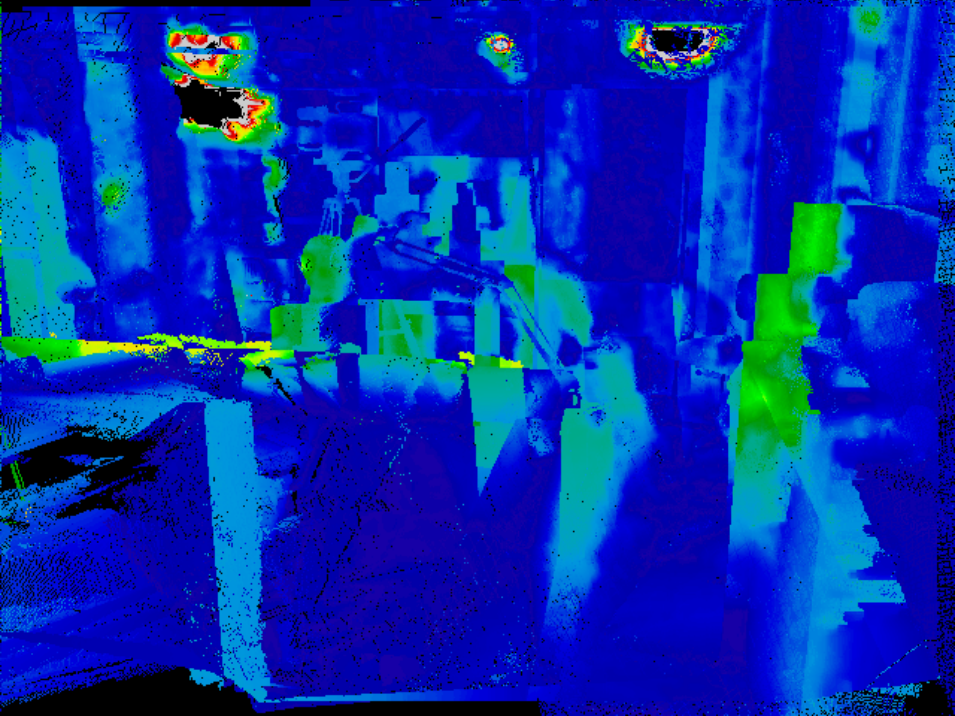
\includegraphics[width=0.2\columnwidth]{./images/tsukuba_frame1314_error_high6.png}%
%			\label{tsukuba_frame1314_error}}
%		\\
%		\subfloat[]{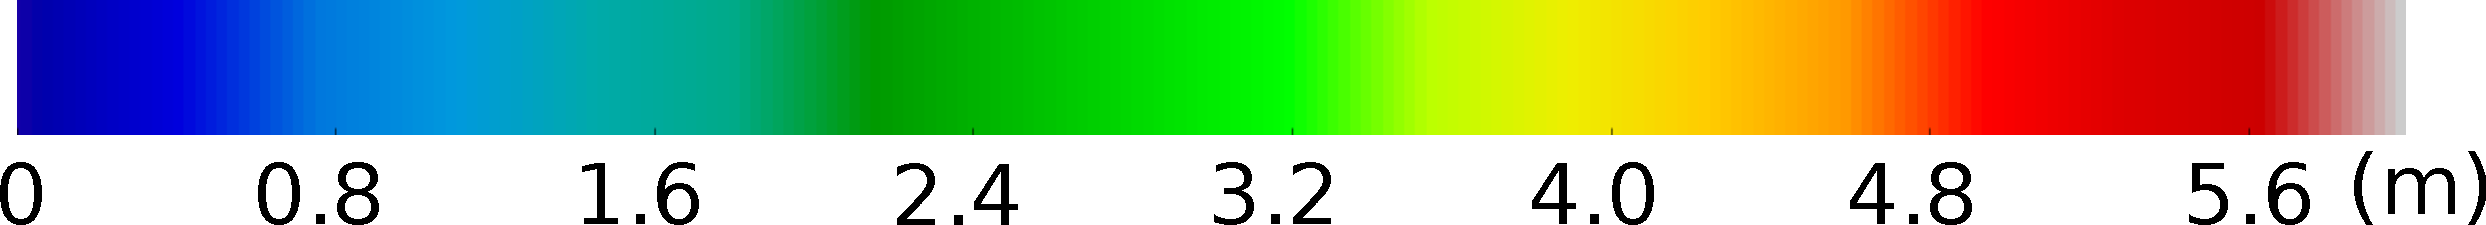
\includegraphics[width=0.4\columnwidth]{./images/high6_bar.pdf}%
%			\label{tsukuba_frame1314_bar}}
%		\caption{Comparison: LIBELAS, DS-PTAM dmaps against GT (Tsukuba)}
%		\label{fig:tsukuba_frame1314}
%	\end{figure}
%\end{frame}

%\begin{frame}
%	\frametitle{KITTI error}
%	\begin{figure}[!htb]
%		\centering
%		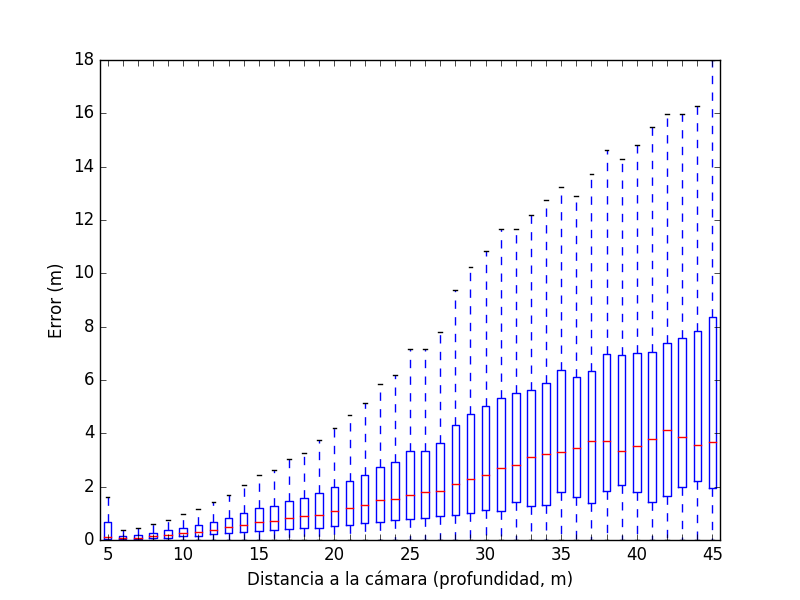
\includegraphics[width=0.33\columnwidth]{images/kitti06_libelas_boxplot}
%		\caption{LIBELAS errors (depth vs errors) on KITTI sequence 06.}
%		\label{fig:kitti06_libelas_boxplot}
%	\end{figure}
%	
%	\begin{figure}[!htb]
%		\centering
%		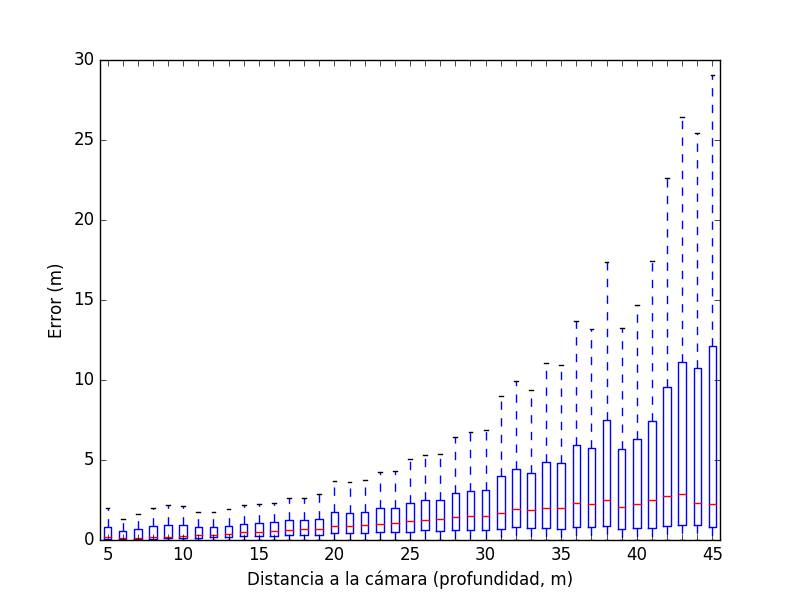
\includegraphics[width=0.33\columnwidth]{images/kitti06_dense_boxplot}
%		\caption{Dense S-PTAM errors (depth vs errors) on KITTI sequence 06.}
%		\label{fig:kitti06_dense_boxplot}
%	\end{figure}
%\end{frame}

\begin{frame}
	\frametitle{KITTI: error de mediana}
	\begin{figure}[!htb]
		\centering
		\includegraphics[width=0.8\columnwidth]{images/medians_comparison_kitti}
		\caption{Median error comparison between LIBELAS and dense (depth vs errors) on KITTI sequence 06.}
		\label{fig:median_comparison_kitti}
	\end{figure}
\end{frame}

%\begin{frame}
%	\frametitle{Tsukuba error}
%	\begin{figure}[!htb]
%		\centering
%		\includegraphics[width=0.33\columnwidth]{images/tsukuba_libelas_boxplot}
%		%\caption{LIBELAS raw reconstruction errors (depth vs errors) in dataset Tsukuba.}
%		\label{fig:tsukuba_libelas_boxplot}
%	\end{figure}
%	\begin{figure}[!htb]
%		\centering
%		\includegraphics[width=0.33\columnwidth]{images/tsukuba_dense_boxplot}
%		%\caption{Errors (depth vs errors) in dataset Tsukuba.}
%		\label{fig:tsukuba_dense_boxplot}
%	\end{figure}
%\end{frame}

\begin{frame}
	\frametitle{Tsukuba: error de mediana}
	\begin{figure}[!htb]
		\centering
		\includegraphics[width=0.8\columnwidth]{images/medians_comparison_tsukuba}
		%\caption{Median error comparison between LIBELAS and Dense S-PTAM (depth vs errors) on Tsukuba sequence.}
		\label{fig:median_comparison_tsukuba}
	\end{figure}
\end{frame}

\begin{frame}
	\frametitle{Cantidad de puntos}
	\begin{figure}[!htb]
		\centering
		\subfloat[KITTI]{\includegraphics[width=0.45\columnwidth]{./images/points_kitti06}%
			\label{tsukuba_frame1314_rgb}}
		\hfil
		\subfloat[Tsukuba]{\includegraphics[width=0.45\columnwidth]{./images/points_tsukuba}%
			\label{tsukuba_frame1314_gt}}
	\end{figure}
\end{frame}
	
%\begin{frame}
%	\frametitle{Cantidad de puntos}
%	\begin{figure}[!htb]
%		\centering
%		\includegraphics[width=\columnwidth]{images/points_kitti06}
%		\caption{Total amount of points during the Dense S-PTAM execution (generated, discarded, present on final reconstruction---hypotheses (saw one time) and validated (fused multiple times)---, and number of fusions) on KITTI 06 sequence.}
%		\label{fig:points_kitti}
%	\end{figure}
%\end{frame}
%
%\begin{frame}
%	\frametitle{Cantidad de puntos}
%\begin{figure}[!htb]
%	\centering
%	\includegraphics[width=\columnwidth]{images/points_tsukuba}
%	\caption{Total amount of points during the Dense S-PTAM execution (generated, discarded, present on final reconstruction---hypotheses (saw one time) and validated (fused multiple times)---, and number of fusions) on Tsukuba sequence.}
%	\label{fig:points_tsukuba}
%\end{figure}
%\end{frame}

\begin{frame}
	\frametitle{Análisis de tiempos}
	\begin{table}[!htb]
		\centering
		\small
		\begin{tabular}{cccc}
			\toprule
			Sequence & Disparity (ms) & Map Fusion (ms) & Map Refinement (ms) \\
			\midrule
			KITTI 06 & 202.66 & 124.76 & 8.00 \\
			Tsukuba & 98.88 & 127.10 & 1.66 \\
			\bottomrule
		\end{tabular}
		\caption{Average computation times (in ms) for each of the main steps of our algorithm.} \label{table:table_times}
	\end{table}
\end{frame}

\begin{frame}
	\frametitle{S-PTAM Denso!}
	\centering
	
	\inlineMovie[loop&autostart&start=5]{./videos/sptam_dense_online.mp4}{./images/kitti_3d_2}{width=\columnwidth}
\end{frame}

\begin{frame}
	\frametitle{S-PTAM Denso!}
	\centering
	
	\inlineMovie[loop&autostart&start=5]{./videos/sptam_dense_offline.mp4}{./images/kitti_3d_2}{width=\columnwidth}
\end{frame}

\section{Conclusiones}

\begin{frame}
	\frametitle{Conclusiones}
	\begin{itemize}
		\item Sistema de SLAM capaz de generar un \textbf{mapa local denso} en \textbf{tiempo real}.
        \item La precisión resulta útil para tareas de \textbf{navegación}.
        \item Evaluado en datasets públicos: KITTI (outdoors) y Tsukuba (indoors).
        \item Funciona incluso en trajectorias largas.
        \item Integrado a S-PTAM y ROS.
	\end{itemize}
\end{frame}


\section*{}

\begin{frame}
	\centering
	\Large{Muchísimas gracias!}
	
	\pause{Preguntas?}
	
	\vspace{2cm}
	Contacto: {\tt pire@cifasis-conicet.gov.ar}
\end{frame}



%%%%%%%%%%%%%%%%%%%%%%%%%%%%%%%%%%%%%%%%%%%%%%%%%%%%%%
%% SLIDES FUERA DE LA PRESENTACIÓN
%%%%%%%%%%%%%%%%%%%%%%%%%%%%%%%%%%%%%%%%%%%%%%%%%%%%%%





\end{document}
